\documentclass[nolineno]{ieeeaccess}
\usepackage{cite}
\usepackage{url}
\usepackage{amsmath,amssymb,amsfonts}
\usepackage{algorithmic}
\usepackage{graphicx}
\usepackage{textcomp}
\def\BibTeX{{\rm B\kern-.05em{\sc i\kern-.025em b}\kern-.08em
    T\kern-.1667em\lower.7ex\hbox{E}\kern-.125emX}}
% Suppress sample volume/year printed by the template on unpublished manuscripts.
\makeatletter
\newcommand{\draftfooters}{%
  \def\@oddfoot{\hfil{\footerpagefont\thepage}}%
  \def\@evenfoot{{\footerpagefont\thepage}\hfil}}
\g@addto@macro\ps@headings{\draftfooters}
\g@addto@macro\ps@titlepage{\draftfooters}
\makeatother
\begin{document}
\pagestyle{headings}
\def\xfigwd{\columnwidth}
\graphicspath{{figures/}{./}}
\newcommand{\RevisionSeeds}{5}
\newcommand{\RevisionRounds}{6}
\newcommand{\RevisionEpochs}{1}
\newcommand{\RevisionBatch}{256}
\newcommand{\RevisionLr}{0.001}
\newcommand{\RevisionWidthA}{64}
\newcommand{\RevisionWidthB}{32}
\newcommand{\RevisionDropout}{0.2}
\newcommand{\RevisionBg}{100}
\newcommand{\RevisionSample}{200}
\newcommand{\RevisionBootstrap}{200}
\newcommand{\RevisionAvgF}{0.6376}
\newcommand{\RevisionAvgB}{0.0161}
\newcommand{\RevisionPerF}{0.8726}
\newcommand{\RevisionPerB}{0.7180}
\newcommand{\RevisionLocalF}{0.9626}
\newcommand{\RevisionLocalB}{0.9965}
\newcommand{\RevisionFixedF}{0.9604}
\newcommand{\RevisionFixedB}{0.9827}
\newcommand{\RevisionAdaptiveF}{0.9634}
\newcommand{\RevisionAdaptiveB}{0.9944}
\newcommand{\RevisionEqualF}{0.9097}
\newcommand{\RevisionEqualB}{0.9592}
\newcommand{\RevisionBalancedF}{0.7116}
\newcommand{\RevisionBalancedB}{0.2478}
\newcommand{\RevisionShortcut}{94.2330}
\newcommand{\RevisionHeadDepthOne}{0.1159}
\newcommand{\RevisionHeadDepthTwo}{0.9922}
\newcommand{\RevisionPerLo}{0.5130}
\newcommand{\RevisionPerHi}{0.5586}
\newcommand{\RevisionProbeAvgB}{0.0161}
\newcommand{\RevisionProbeAvgA}{0.9982}
\newcommand{\RevisionProbeAvgBrier}{0.3891}
\newcommand{\RevisionPlattB}{0.8370}
\newcommand{\RevisionPlattA}{0.9084}
\newcommand{\RevisionPlattBrier}{0.1007}
\newcommand{\RevisionTemperatureB}{0.0161}
\newcommand{\RevisionTemperatureA}{0.9982}
\newcommand{\RevisionTemperatureBrier}{0.2393}
\newcommand{\RevisionThresholdB}{0.9619}
\newcommand{\RevisionThresholdA}{0.3253}
\newcommand{\RevisionThresholdBrier}{0.3891}
\newcommand{\RevisionHeadB}{0.2577}
\newcommand{\RevisionHeadA}{0.9873}
\newcommand{\RevisionHeadBrier}{0.2332}
\newcommand{\RevisionTuneB}{0.9903}
\newcommand{\RevisionTuneA}{0.9589}
\newcommand{\RevisionTuneBrier}{0.0220}
\newcommand{\RevisionCka}{0.9720}
\newcommand{\RevisionWithinAttack}{0.9843}
\newcommand{\RevisionWithinBenign}{0.9835}
\newcommand{\RevisionAcrossAttack}{0.2450}

\newcommand{\RevisionTaxonomy}{%
\begin{table*}[t]\centering
\caption{Attack labels and potential service consequences in the derived subset.}\label{tab:attacks}
\resizebox{\textwidth}{!}{\begin{tabular}{lrrrr}\hline
Label & Client & Records & Possible service impact & Source\\\hline
BT-DoS & bluetooth & 6,735 & Gaps in wearable observations & \cite{dadkhah2024towards}\\
MQTT-DDoS-Connect\_Flood & mqtt & 17,264 & Less broker capacity for legitimate sessions & \cite{dadkhah2024towards}\\
MQTT-DDoS-Publish\_Flood & mqtt & 4,179 & Delayed monitoring topic updates & \cite{dadkhah2024towards}\\
MQTT-DoS-Connect\_Flood & mqtt & 2,707 & Less broker capacity for legitimate sessions & \cite{dadkhah2024towards}\\
MQTT-DoS-Publish\_Flood & mqtt & 5,411 & Delayed monitoring topic updates & \cite{dadkhah2024towards}\\
MQTT-Malformed\_Data & mqtt & 2,047 & Application endpoint processing errors & \cite{dadkhah2024towards}\\
ARP\_Spoofing & wifi & 1,584 & Misdirection of gateway-bound telemetry & \cite{dadkhah2024towards}\\
Recon-OS\_Scan & wifi & 1,611 & Discovery of exposed monitoring services & \cite{dadkhah2024towards}\\
Recon-Ping\_Sweep & wifi & 926 & Discovery of exposed monitoring services & \cite{dadkhah2024towards}\\
Recon-Port\_Scan & wifi & 2,432 & Discovery of exposed monitoring services & \cite{dadkhah2024towards}\\
Recon-VulScan & wifi & 1,444 & Discovery of exposed monitoring services & \cite{dadkhah2024towards}\\
TCP\_IP-DDoS-ICMP & wifi & 19,440 & Contention with monitor traffic & \cite{dadkhah2024towards}\\
TCP\_IP-DDoS-SYN & wifi & 10,721 & Contention with monitor traffic & \cite{dadkhah2024towards}\\
TCP\_IP-DDoS-TCP & wifi & 10,842 & Contention with monitor traffic & \cite{dadkhah2024towards}\\
TCP\_IP-DDoS-UDP & wifi & 20,498 & Contention with monitor traffic & \cite{dadkhah2024towards}\\
TCP\_IP-DoS-ICMP & wifi & 6,330 & Contention with monitor traffic & \cite{dadkhah2024towards}\\
TCP\_IP-DoS-SYN & wifi & 6,577 & Contention with monitor traffic & \cite{dadkhah2024towards}\\
TCP\_IP-DoS-TCP & wifi & 5,831 & Contention with monitor traffic & \cite{dadkhah2024towards}\\
TCP\_IP-DoS-UDP & wifi & 8,143 & Contention with monitor traffic & \cite{dadkhah2024towards}\\
\hline\end{tabular}}
\end{table*}
}

\newcommand{\RevisionTopology}{%
\begin{figure*}[t]\centering
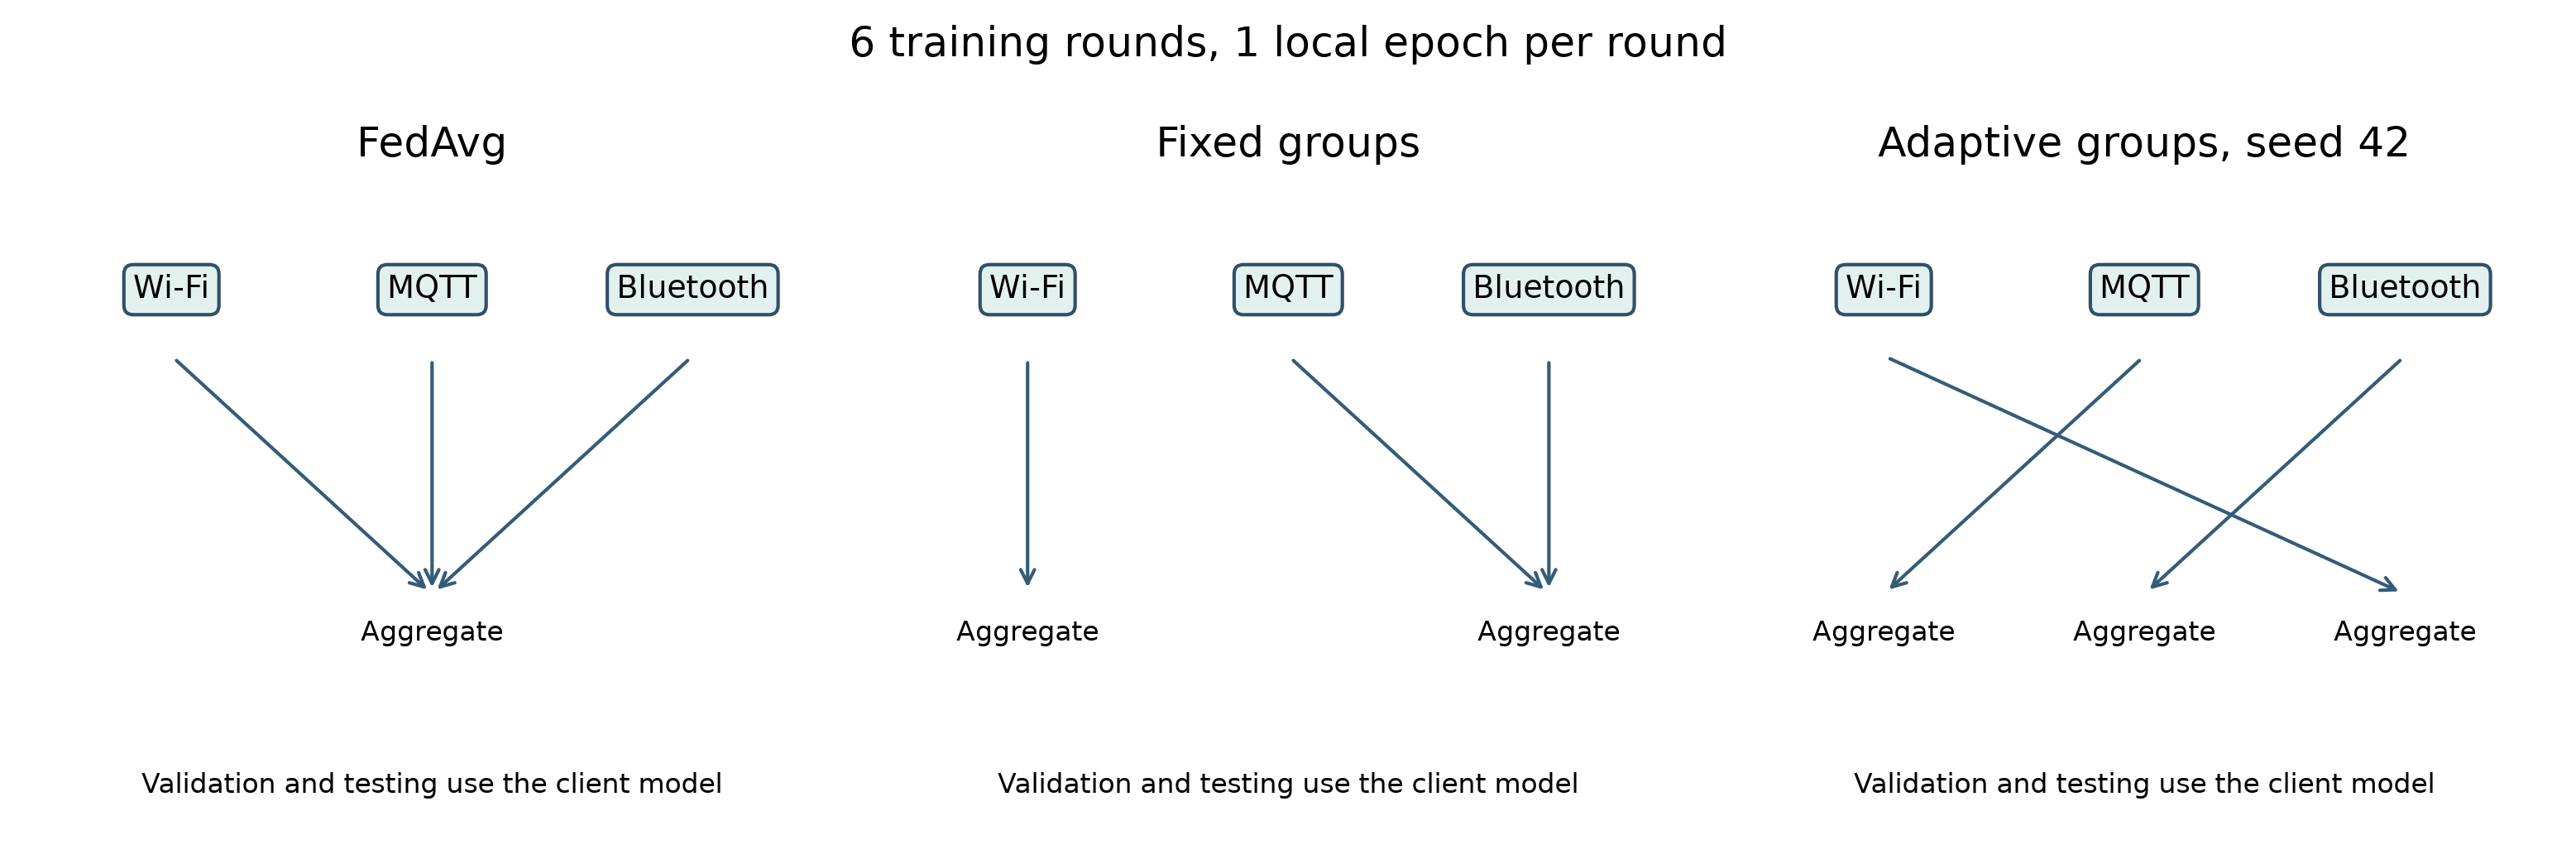
\includegraphics[width=0.93\textwidth]{revision_topology.png}
\caption{Training and parameter exchange by aggregation policy. Raw features stay with each simulated client during federated training. FedPer additionally retains its classification head locally. Pooled training is an offline comparator.}\label{fig:revised_topology}
\end{figure*}

\begin{table}[t]\centering
\caption{Adaptive group membership at each validation-selected checkpoint.}\label{tab:newgroups}
\small\begin{tabular}{lr}\hline
Seed & Client grouping\\\hline
42 & mqtt / bluetooth / wifi\\
7 & mqtt / bluetooth / wifi\\
123 & mqtt / bluetooth / wifi\\
2024 & mqtt / bluetooth / wifi\\
31337 & mqtt / bluetooth / wifi\\
\hline\end{tabular}
\end{table}
}

\newcommand{\RevisionDetection}{%
\begin{table*}[t]\centering
\caption{Grouped evaluation across 5 matched seeds. Entries are means and sample standard deviations.}\label{tab:newmain}
\resizebox{\textwidth}{!}{\begin{tabular}{lrrrr}\hline
Method & Client mean macro F1 & Pooled macro F1 & Bluetooth benign recall & Optimizer steps\\\hline
Adaptive groups & 0.9634 $\pm$ 0.0020 & 0.9768 $\pm$ 0.0014 & 0.9944 $\pm$ 0.0017 & 2349.6000 $\pm$ 3.2863\\
Centralized & 0.9639 $\pm$ 0.0022 & 0.9772 $\pm$ 0.0014 & 0.9963 $\pm$ 0.0014 & 2347.2000 $\pm$ 2.6833\\
Compute-matched centralized & 0.9641 $\pm$ 0.0024 & 0.9772 $\pm$ 0.0015 & 0.9964 $\pm$ 0.0013 & 2349.6000 $\pm$ 3.2863\\
Class-balanced loss & 0.7116 $\pm$ 0.0671 & 0.7878 $\pm$ 0.0395 & 0.2478 $\pm$ 0.2542 & 2349.6000 $\pm$ 3.2863\\
Equal client weights & 0.9097 $\pm$ 0.0021 & 0.9266 $\pm$ 0.0038 & 0.9592 $\pm$ 0.0084 & 2349.6000 $\pm$ 3.2863\\
FedAvg & 0.6376 $\pm$ 0.0458 & 0.7022 $\pm$ 0.0677 & 0.0161 $\pm$ 0.0214 & 2349.6000 $\pm$ 3.2863\\
FedPer & 0.8726 $\pm$ 0.0242 & 0.8949 $\pm$ 0.0196 & 0.7180 $\pm$ 0.1016 & 2349.6000 $\pm$ 3.2863\\
FedProx 0.001 & 0.6818 $\pm$ 0.0179 & 0.7667 $\pm$ 0.0105 & 0.0350 $\pm$ 0.0387 & 2349.6000 $\pm$ 3.2863\\
FedProx 0.01 & 0.6836 $\pm$ 0.0085 & 0.7820 $\pm$ 0.0050 & 0.0214 $\pm$ 0.0191 & 2349.6000 $\pm$ 3.2863\\
FedProx 0.05 & 0.6751 $\pm$ 0.0062 & 0.7779 $\pm$ 0.0068 & 0.0157 $\pm$ 0.0111 & 2349.6000 $\pm$ 3.2863\\
FedProx 0.1 & 0.6697 $\pm$ 0.0060 & 0.7725 $\pm$ 0.0080 & 0.0137 $\pm$ 0.0105 & 2349.6000 $\pm$ 3.2863\\
FedProx 0 & 0.6376 $\pm$ 0.0458 & 0.7022 $\pm$ 0.0677 & 0.0161 $\pm$ 0.0214 & 2349.6000 $\pm$ 3.2863\\
Fixed groups & 0.9604 $\pm$ 0.0026 & 0.9755 $\pm$ 0.0014 & 0.9827 $\pm$ 0.0028 & 2349.6000 $\pm$ 3.2863\\
Local-only & 0.9626 $\pm$ 0.0017 & 0.9768 $\pm$ 0.0012 & 0.9965 $\pm$ 0.0014 & 2349.6000 $\pm$ 3.2863\\
\hline\end{tabular}}
\end{table*}

\begin{table*}[t]\centering
\caption{Grouped test results for seed 42. BT denotes Bluetooth.}\label{tab:newseed42}
\resizebox{\textwidth}{!}{\begin{tabular}{lrrrrrrr}\hline
Method & Wi-Fi F1 & MQTT F1 & BT F1 & Wi-Fi benign & MQTT benign & BT benign & Client mean\\\hline
Adaptive groups & 0.9363 & 0.9694 & 0.9841 & 0.8368 & 0.9700 & 0.9947 & 0.9633\\
Centralized & 0.9359 & 0.9697 & 0.9867 & 0.8148 & 0.9628 & 0.9973 & 0.9641\\
Compute-matched centralized & 0.9359 & 0.9697 & 0.9867 & 0.8148 & 0.9628 & 0.9973 & 0.9641\\
Class-balanced loss & 0.8351 & 0.8218 & 0.4043 & 0.9986 & 0.6336 & 0.1151 & 0.6871\\
Equal client weights & 0.8549 & 0.9077 & 0.9643 & 0.9835 & 0.8101 & 0.9570 & 0.9090\\
FedAvg & 0.9201 & 0.7533 & 0.3022 & 0.9438 & 0.4710 & 0.0106 & 0.6586\\
FedPer & 0.9324 & 0.8375 & 0.7223 & 0.8848 & 0.6440 & 0.5459 & 0.8307\\
FedProx 0.001 & 0.9140 & 0.7913 & 0.2942 & 0.9492 & 0.5400 & 0.0032 & 0.6665\\
FedProx 0.01 & 0.9065 & 0.8268 & 0.2942 & 0.9630 & 0.6093 & 0.0032 & 0.6758\\
FedProx 0.05 & 0.8897 & 0.8144 & 0.2981 & 0.9767 & 0.5905 & 0.0069 & 0.6674\\
FedProx 0.1 & 0.8872 & 0.8020 & 0.2968 & 0.9753 & 0.5721 & 0.0058 & 0.6620\\
FedProx 0 & 0.9201 & 0.7533 & 0.3022 & 0.9438 & 0.4710 & 0.0106 & 0.6586\\
Fixed groups & 0.9362 & 0.9705 & 0.9750 & 0.8505 & 0.9856 & 0.9830 & 0.9606\\
Local-only & 0.9345 & 0.9705 & 0.9831 & 0.8395 & 0.9735 & 0.9979 & 0.9627\\
\hline\end{tabular}}
\end{table*}

\begin{table*}[t]\centering
\caption{Grouped test results for seed 7. BT denotes Bluetooth.}\label{tab:newseed7}
\resizebox{\textwidth}{!}{\begin{tabular}{lrrrrrrr}\hline
Method & Wi-Fi F1 & MQTT F1 & BT F1 & Wi-Fi benign & MQTT benign & BT benign & Client mean\\\hline
Adaptive groups & 0.9352 & 0.9760 & 0.9846 & 0.8230 & 0.9850 & 0.9949 & 0.9652\\
Centralized & 0.9365 & 0.9763 & 0.9842 & 0.8385 & 0.9780 & 0.9974 & 0.9657\\
Compute-matched centralized & 0.9382 & 0.9764 & 0.9855 & 0.8385 & 0.9790 & 0.9974 & 0.9667\\
Class-balanced loss & 0.8451 & 0.8122 & 0.5926 & 0.9986 & 0.6092 & 0.3524 & 0.7500\\
Equal client weights & 0.8489 & 0.9170 & 0.9701 & 0.9705 & 0.8353 & 0.9645 & 0.9120\\
FedAvg & 0.8975 & 0.7338 & 0.2870 & 0.9143 & 0.4397 & 0.0005 & 0.6395\\
FedPer & 0.9291 & 0.8643 & 0.8782 & 0.8596 & 0.7092 & 0.8138 & 0.8905\\
FedProx 0.001 & 0.9045 & 0.7954 & 0.2886 & 0.9129 & 0.5499 & 0.0021 & 0.6629\\
FedProx 0.01 & 0.8940 & 0.8383 & 0.2880 & 0.9129 & 0.6334 & 0.0015 & 0.6734\\
FedProx 0.05 & 0.8717 & 0.8502 & 0.2876 & 0.9256 & 0.6584 & 0.0010 & 0.6698\\
FedProx 0.1 & 0.8672 & 0.8441 & 0.2882 & 0.9368 & 0.6490 & 0.0015 & 0.6665\\
FedProx 0 & 0.8975 & 0.7338 & 0.2870 & 0.9143 & 0.4397 & 0.0005 & 0.6395\\
Fixed groups & 0.9357 & 0.9743 & 0.9798 & 0.8216 & 0.9962 & 0.9866 & 0.9633\\
Local-only & 0.9366 & 0.9762 & 0.9820 & 0.8301 & 0.9890 & 0.9974 & 0.9649\\
\hline\end{tabular}}
\end{table*}

\begin{table*}[t]\centering
\caption{Source-label supports and binary detector recall, seed 42.}\label{tab:newsupport}
\resizebox{\textwidth}{!}{\begin{tabular}{lrrrrrr}\hline
Label & Client & Train & Validation & Test & FedAvg recall & FedPer recall\\\hline
BT-DoS & bluetooth & 4075 & 1352 & 1308 & 0.9992 & 0.9809\\
Benign & bluetooth & 5800 & 1926 & 1885 & 0.0106 & 0.5459\\
Benign & mqtt & 10970 & 3680 & 3739 & 0.4710 & 0.6440\\
MQTT-DDoS-Connect\_Flood & mqtt & 10410 & 3357 & 3497 & 1.0000 & 1.0000\\
MQTT-DDoS-Publish\_Flood & mqtt & 2440 & 849 & 890 & 1.0000 & 1.0000\\
MQTT-DoS-Connect\_Flood & mqtt & 1593 & 568 & 546 & 1.0000 & 1.0000\\
MQTT-DoS-Publish\_Flood & mqtt & 3212 & 1105 & 1094 & 1.0000 & 1.0000\\
MQTT-Malformed\_Data & mqtt & 1202 & 422 & 423 & 0.9905 & 0.8251\\
ARP\_Spoofing & wifi & 956 & 312 & 316 & 0.7247 & 0.8259\\
Benign & wifi & 2169 & 716 & 729 & 0.9438 & 0.8848\\
Recon-OS\_Scan & wifi & 1006 & 294 & 311 & 0.9035 & 0.9293\\
Recon-Ping\_Sweep & wifi & 533 & 214 & 179 & 0.7877 & 0.9665\\
Recon-Port\_Scan & wifi & 1417 & 529 & 486 & 0.9691 & 0.9794\\
Recon-VulScan & wifi & 900 & 278 & 266 & 0.8722 & 0.9398\\
TCP\_IP-DDoS-ICMP & wifi & 11963 & 3606 & 3871 & 1.0000 & 1.0000\\
TCP\_IP-DDoS-SYN & wifi & 6449 & 2147 & 2125 & 0.9995 & 1.0000\\
TCP\_IP-DDoS-TCP & wifi & 6445 & 2278 & 2119 & 1.0000 & 1.0000\\
TCP\_IP-DDoS-UDP & wifi & 12345 & 4059 & 4094 & 0.9998 & 1.0000\\
TCP\_IP-DoS-ICMP & wifi & 3866 & 1215 & 1249 & 1.0000 & 1.0000\\
TCP\_IP-DoS-SYN & wifi & 3953 & 1324 & 1300 & 0.9992 & 1.0000\\
TCP\_IP-DoS-TCP & wifi & 3526 & 1142 & 1163 & 1.0000 & 1.0000\\
TCP\_IP-DoS-UDP & wifi & 4876 & 1619 & 1648 & 0.9994 & 1.0000\\
\hline\end{tabular}}
\end{table*}
}

\newcommand{\RevisionBudget}{%
\begin{figure*}[t]\centering
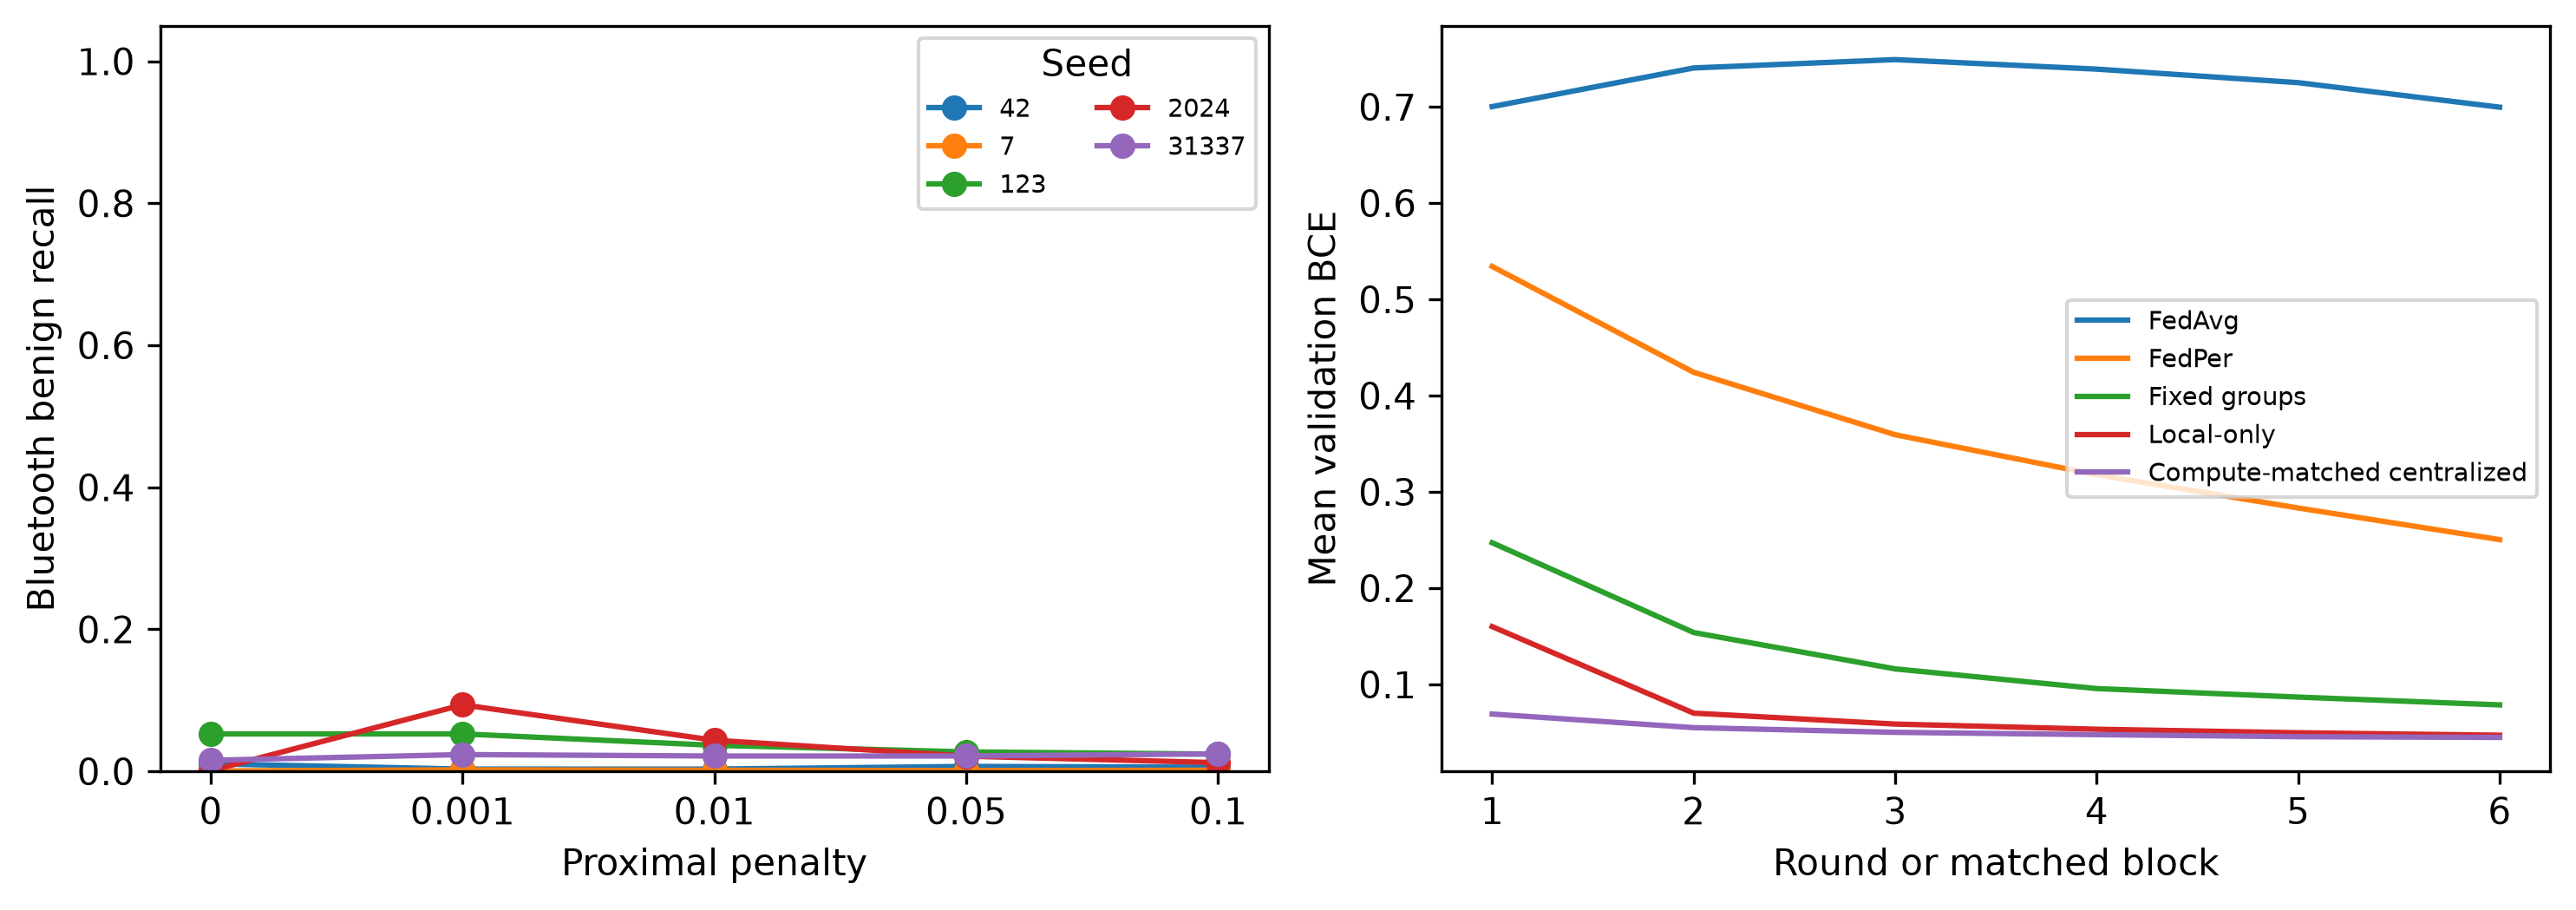
\includegraphics[width=0.93\textwidth]{revision_sweep_budget.png}
\caption{Left: test specificity for the proximal sweep. Right: validation binary cross-entropy averaged over clients and seeds.}\label{fig:revised_sweep_budget}
\end{figure*}
}

\newcommand{\RevisionDiagnostics}{%
\begin{table*}[t]\centering
\caption{Bluetooth diagnostics on 5 seeds, mean and sample standard deviation.}\label{tab:newprobe}
\resizebox{\textwidth}{!}{\begin{tabular}{lrrrrrr}\hline
Model & Specificity & Attack recall & Brier & ECE & ROC AUC & PR AUC\\\hline
fedavg & 0.0161 $\pm$ 0.0214 & 0.9982 $\pm$ 0.0022 & 0.3891 $\pm$ 0.0333 & 0.4602 $\pm$ 0.0338 & 0.8956 $\pm$ 0.0828 & 0.7576 $\pm$ 0.1452\\
threshold & 0.9619 $\pm$ 0.0190 & 0.3253 $\pm$ 0.4386 & 0.3891 $\pm$ 0.0333 & 0.4602 $\pm$ 0.0338 & 0.8956 $\pm$ 0.0828 & 0.7576 $\pm$ 0.1452\\
platt & 0.8370 $\pm$ 0.0952 & 0.9084 $\pm$ 0.0902 & 0.1007 $\pm$ 0.0470 & 0.1205 $\pm$ 0.0666 & 0.8956 $\pm$ 0.0828 & 0.7576 $\pm$ 0.1452\\
temperature & 0.0161 $\pm$ 0.0214 & 0.9982 $\pm$ 0.0022 & 0.2393 $\pm$ 0.0089 & 0.2933 $\pm$ 0.1007 & 0.8956 $\pm$ 0.0828 & 0.7576 $\pm$ 0.1452\\
fedper & 0.7180 $\pm$ 0.1016 & 0.9771 $\pm$ 0.0058 & 0.1297 $\pm$ 0.0287 & 0.2477 $\pm$ 0.0251 & 0.9739 $\pm$ 0.0091 & 0.9488 $\pm$ 0.0409\\
frozen trunk & 0.2577 $\pm$ 0.2387 & 0.9873 $\pm$ 0.0071 & 0.2332 $\pm$ 0.0322 & 0.3393 $\pm$ 0.0245 & 0.9624 $\pm$ 0.0272 & 0.9173 $\pm$ 0.0893\\
fine tune & 0.9903 $\pm$ 0.0045 & 0.9589 $\pm$ 0.0036 & 0.0220 $\pm$ 0.0027 & 0.0294 $\pm$ 0.0147 & 0.9810 $\pm$ 0.0031 & 0.9848 $\pm$ 0.0021\\
\hline\end{tabular}}
\end{table*}

\begin{figure*}[t]\centering
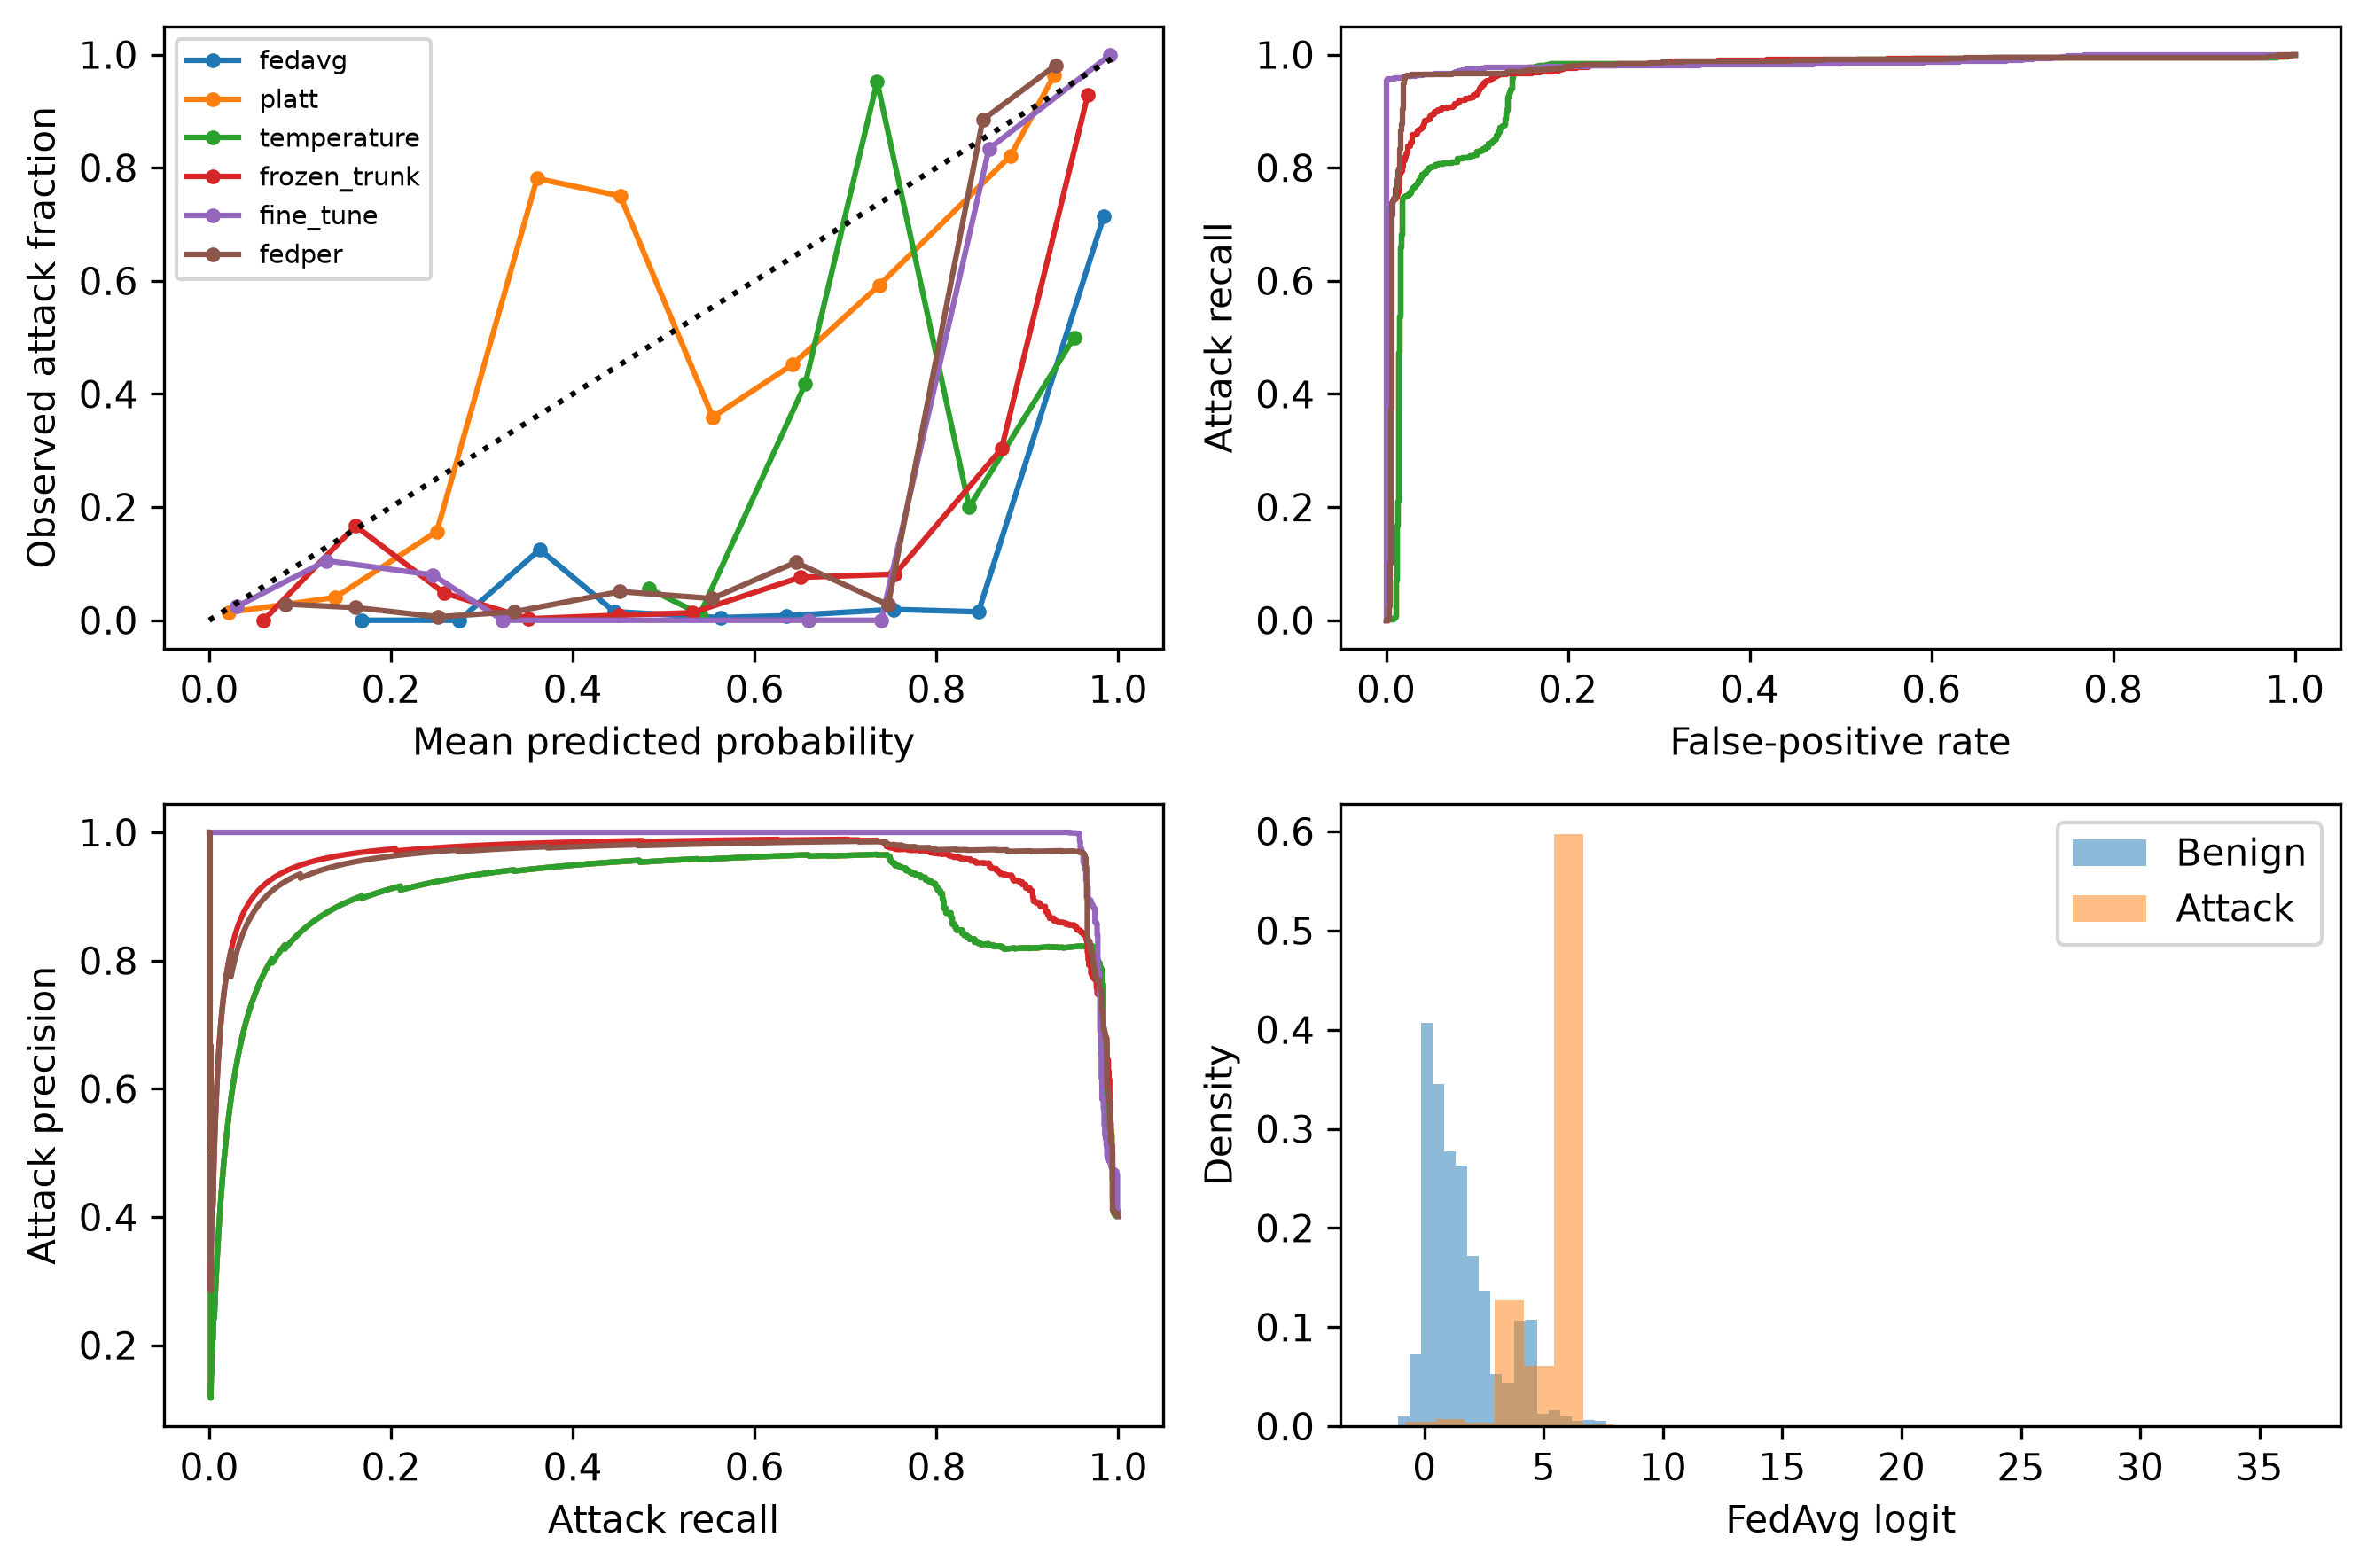
\includegraphics[width=0.93\textwidth]{revision_diagnostic.png}
\caption{Bluetooth score diagnostics for seed 123. Reliability, receiver operating characteristic, precision--recall, and the class-conditional FedAvg scores.}\label{fig:revised_diagnostic}
\end{figure*}
}

\newcommand{\RevisionShap}{%
\begin{table}[t]\centering
\caption{FedPer versus FedAvg within client on matched backgrounds and records.}\label{tab:newshapwithin}
\resizebox{\columnwidth}{!}{\begin{tabular}{lrrr}\hline
Client and class & Top-five Jaccard & Spearman & Cosine\\\hline
wifi benign & 0.6024 $\pm$ 0.2832 & 0.9606 $\pm$ 0.0414 & 0.9824 $\pm$ 0.0164\\
wifi attack & 0.6667 $\pm$ 0.0000 & 0.9521 $\pm$ 0.0400 & 0.9863 $\pm$ 0.0212\\
mqtt benign & 0.5905 $\pm$ 0.2511 & 0.9486 $\pm$ 0.0361 & 0.9810 $\pm$ 0.0205\\
mqtt attack & 0.7524 $\pm$ 0.2461 & 0.8976 $\pm$ 0.0331 & 0.9854 $\pm$ 0.0175\\
bluetooth benign & 0.5548 $\pm$ 0.2896 & 0.9835 $\pm$ 0.0080 & 0.8657 $\pm$ 0.0563\\
bluetooth attack & 0.4881 $\pm$ 0.1786 & 0.9843 $\pm$ 0.0093 & 0.9131 $\pm$ 0.0280\\
\hline\end{tabular}}
\end{table}

\begin{table}[t]\centering
\caption{Within-method comparisons across clients using client-specific backgrounds.}\label{tab:newshapacross}
\resizebox{\columnwidth}{!}{\begin{tabular}{lrrr}\hline
Pair and class & Top-five Jaccard & Spearman & Cosine\\\hline
wifi-mqtt benign & 0.2024 $\pm$ 0.1400 & 0.7968 $\pm$ 0.0224 & 0.9078 $\pm$ 0.0366\\
wifi-mqtt attack & 0.6857 $\pm$ 0.2037 & 0.7236 $\pm$ 0.0301 & 0.9671 $\pm$ 0.0093\\
wifi-bluetooth benign & 0.0444 $\pm$ 0.0609 & 0.4499 $\pm$ 0.0704 & 0.2013 $\pm$ 0.0329\\
wifi-bluetooth attack & 0.0222 $\pm$ 0.0497 & 0.2450 $\pm$ 0.0550 & 0.0947 $\pm$ 0.0096\\
mqtt-bluetooth benign & 0.0000 $\pm$ 0.0000 & 0.3224 $\pm$ 0.0638 & 0.1411 $\pm$ 0.0649\\
mqtt-bluetooth attack & 0.0444 $\pm$ 0.0609 & 0.1557 $\pm$ 0.0825 & 0.1126 $\pm$ 0.0572\\
\hline\end{tabular}}
\end{table}

\begin{figure*}[t]\centering
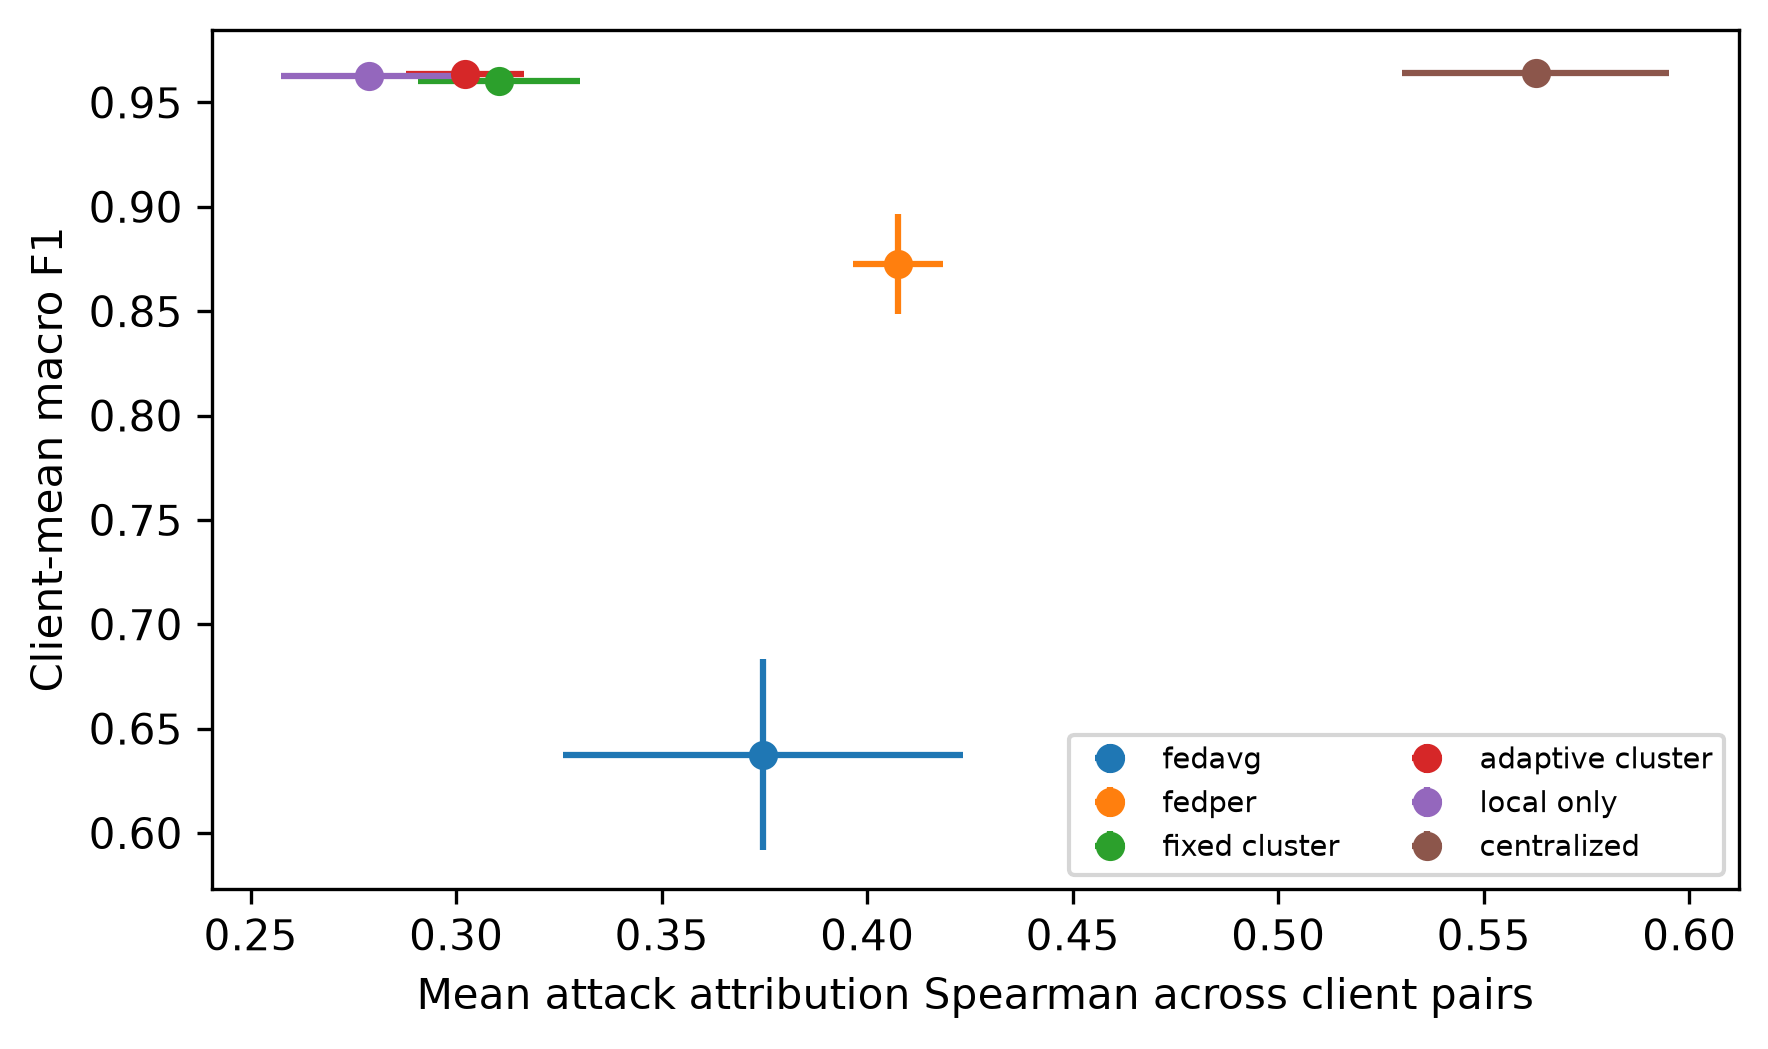
\includegraphics[width=0.93\textwidth]{revision_shap_tradeoff.png}
\caption{Each point averages over the available matched seeds. The horizontal statistic first averages the three within-method protocol pairs. Error bars are sample standard deviations across seeds.}\label{fig:revised_shap_tradeoff}
\end{figure*}
}

\newcommand{\RevisionSensitivity}{%
\begin{table*}[t]\centering
\caption{One-factor settings and the round-by-epoch interaction on the reduced budget.}\label{tab:newsensitivity}
\resizebox{\textwidth}{!}{\begin{tabular}{lrrrr}\hline
Setting & Seeds & Client mean macro F1 & BT specificity & BT Spearman\\\hline
anchor & 2 & 0.5752 $\pm$ 0.0021 & 0.0000 $\pm$ 0.0000 & 0.9927 $\pm$ 0.0009\\
batch 128 & 2 & 0.5989 $\pm$ 0.0023 & 0.0000 $\pm$ 0.0000 & 0.9933 $\pm$ 0.0015\\
batch 512 & 2 & 0.5458 $\pm$ 0.0076 & 0.0000 $\pm$ 0.0000 & 0.9914 $\pm$ 0.0018\\
dropout 0 & 2 & 0.6034 $\pm$ 0.0474 & 0.0003 $\pm$ 0.0004 & 0.9917 $\pm$ 0.0081\\
dropout 04 & 2 & 0.5733 $\pm$ 0.0054 & 0.0000 $\pm$ 0.0000 & 0.9922 $\pm$ 0.0034\\
epochs 1 & 2 & 0.5409 $\pm$ 0.0111 & 0.0000 $\pm$ 0.0000 & 0.9897 $\pm$ 0.0051\\
epochs 3 & 2 & 0.5975 $\pm$ 0.0046 & 0.0000 $\pm$ 0.0000 & 0.9939 $\pm$ 0.0013\\
head 1 & 2 & 0.7025 $\pm$ 0.0349 & 0.1159 $\pm$ 0.1046 & 0.9863 $\pm$ 0.0056\\
head 2 & 2 & 0.9606 $\pm$ 0.0003 & 0.9922 $\pm$ 0.0002 & 0.9760 $\pm$ 0.0083\\
interaction high & 2 & 0.5975 $\pm$ 0.0046 & 0.0000 $\pm$ 0.0000 & 0.9939 $\pm$ 0.0013\\
interaction long short & 2 & 0.6490 $\pm$ 0.0135 & 0.0056 $\pm$ 0.0071 & 1.0000 $\pm$ 0.0000\\
interaction low & 2 & 0.5409 $\pm$ 0.0111 & 0.0000 $\pm$ 0.0000 & 0.9897 $\pm$ 0.0051\\
interaction short long & 2 & 0.5975 $\pm$ 0.0046 & 0.0000 $\pm$ 0.0000 & 0.9939 $\pm$ 0.0013\\
lr high & 2 & 0.6317 $\pm$ 0.0307 & 0.0003 $\pm$ 0.0004 & 0.9948 $\pm$ 0.0010\\
lr low & 2 & 0.5433 $\pm$ 0.0050 & 0.0000 $\pm$ 0.0000 & 0.9914 $\pm$ 0.0018\\
rounds 2 & 2 & 0.5752 $\pm$ 0.0021 & 0.0000 $\pm$ 0.0000 & 0.9927 $\pm$ 0.0009\\
rounds 6 & 2 & 0.6126 $\pm$ 0.0550 & 0.0013 $\pm$ 0.0018 & 0.9933 $\pm$ 0.0017\\
width double & 2 & 0.6086 $\pm$ 0.0108 & 0.0019 $\pm$ 0.0026 & 0.9933 $\pm$ 0.0006\\
width half & 2 & 0.5402 $\pm$ 0.0065 & 0.0000 $\pm$ 0.0000 & 0.9809 $\pm$ 0.0043\\
\hline\end{tabular}}
\end{table*}

\begin{figure*}[t]\centering
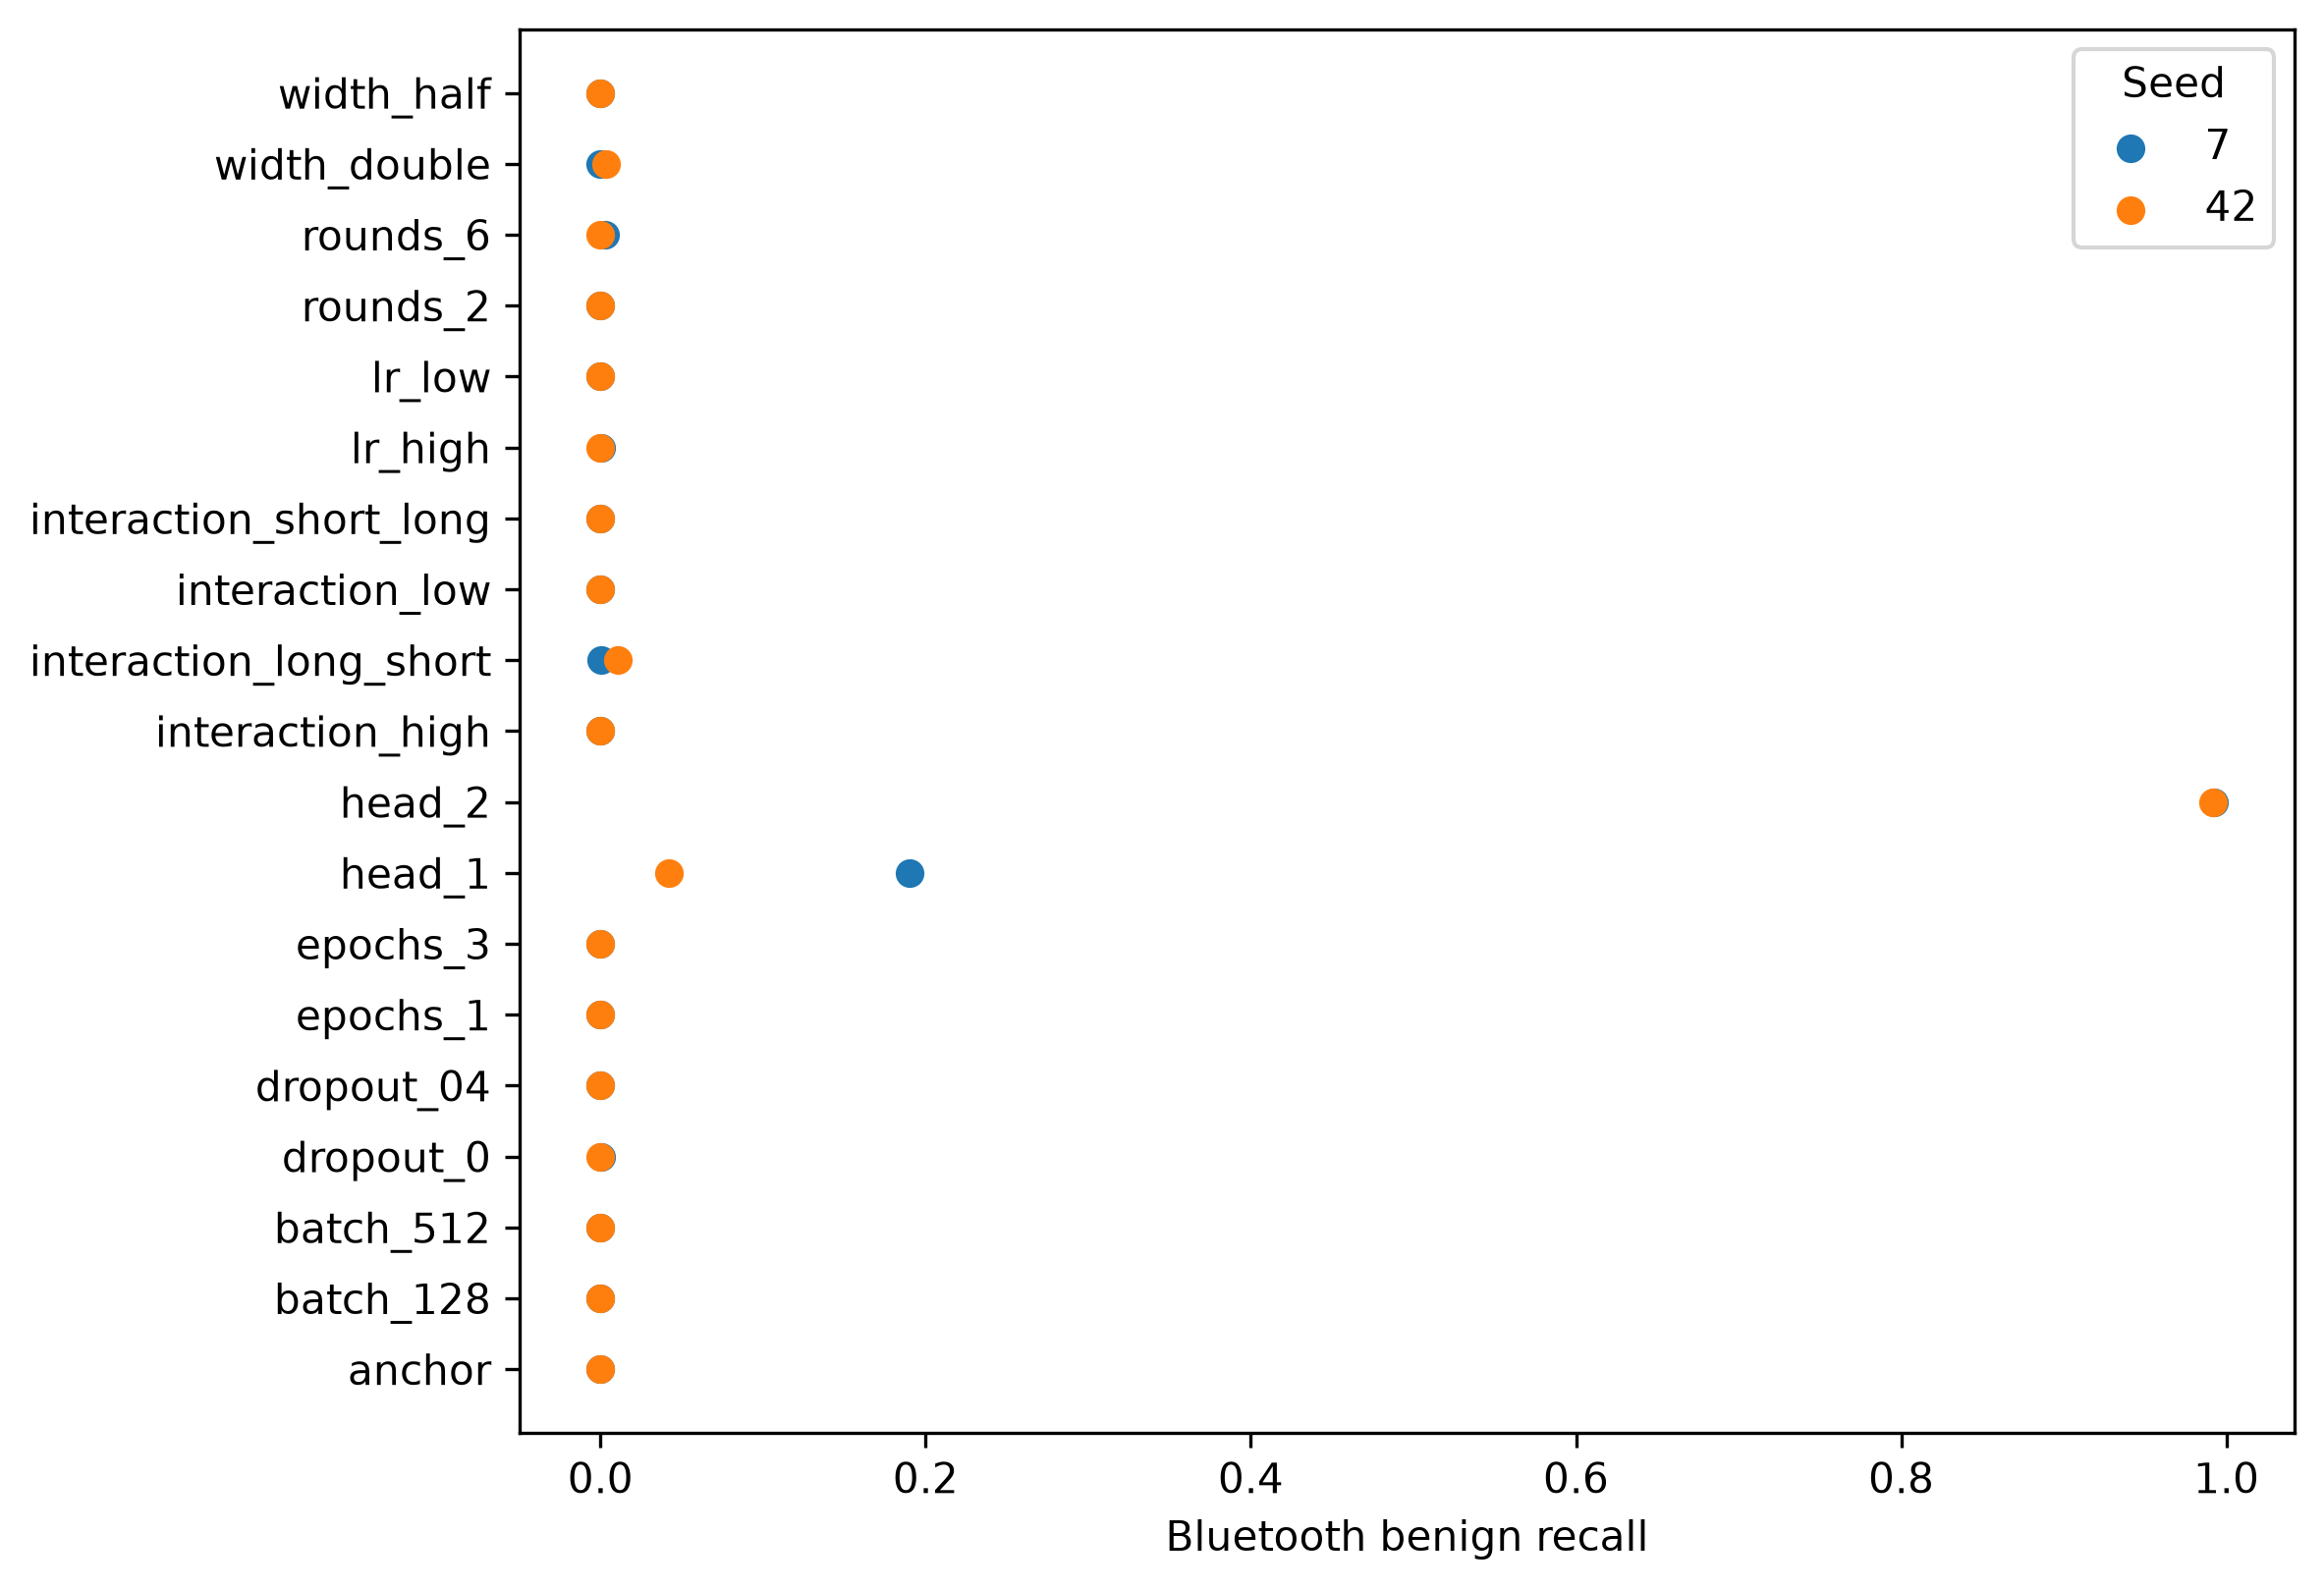
\includegraphics[width=0.93\textwidth]{revision_sensitivity.png}
\caption{Bluetooth benign recall across tested sensitivity configurations.}\label{fig:revised_sensitivity}
\end{figure*}
}

\newcommand{\RevisionTransfer}{%
\begin{table}[t]\centering
\caption{Foreign-feature transfer to the Bluetooth model. Attack metrics weight source labels equally.}\label{tab:newtransfer}
\resizebox{\columnwidth}{!}{\begin{tabular}{lrrr}\hline
Target model & Attack recall & Source-mean benign FPR & Detection margin\\\hline
FedAvg & 0.9915 & 1.0000 & -0.0085\\
FedPer & 0.9031 & 0.9715 & -0.0684\\
Fixed groups & 0.7763 & 0.9537 & -0.1767\\
Adaptive groups & 0.5764 & 0.9505 & -0.3734\\
Local-only & 0.1058 & 0.1643 & -0.0582\\
Centralized & 0.9455 & 0.9882 & -0.0428\\
\hline\end{tabular}}
\end{table}

\begin{table}[t]\centering
\caption{Binary recall on the omitted reconnaissance labels. Each retained test label has equal weight.}\label{tab:newholdout}
\small\begin{tabular}{lrr}\hline
Training method & Seeds & Reconnaissance recall\\\hline
Adaptive groups & 2 & 0.8931 $\pm$ 0.0143\\
Centralized & 2 & 0.9022 $\pm$ 0.0601\\
Compute-matched centralized & 2 & 0.9047 $\pm$ 0.0491\\
Class-balanced loss & 2 & 0.5847 $\pm$ 0.0365\\
Equal client weights & 2 & 0.5967 $\pm$ 0.0214\\
FedAvg & 2 & 0.6824 $\pm$ 0.0315\\
FedPer & 2 & 0.7906 $\pm$ 0.0449\\
FedProx 0 & 2 & 0.6824 $\pm$ 0.0315\\
FedProx 0.001 & 2 & 0.6384 $\pm$ 0.0202\\
FedProx 0.01 & 2 & 0.6362 $\pm$ 0.0222\\
FedProx 0.05 & 2 & 0.6265 $\pm$ 0.0237\\
FedProx 0.1 & 2 & 0.6252 $\pm$ 0.0209\\
Fixed groups & 2 & 0.9027 $\pm$ 0.0225\\
Local-only & 2 & 0.8723 $\pm$ 0.0115\\
\hline\end{tabular}
\end{table}
}

\newcommand{\RevisionScarcity}{%
\begin{figure*}[t]\centering
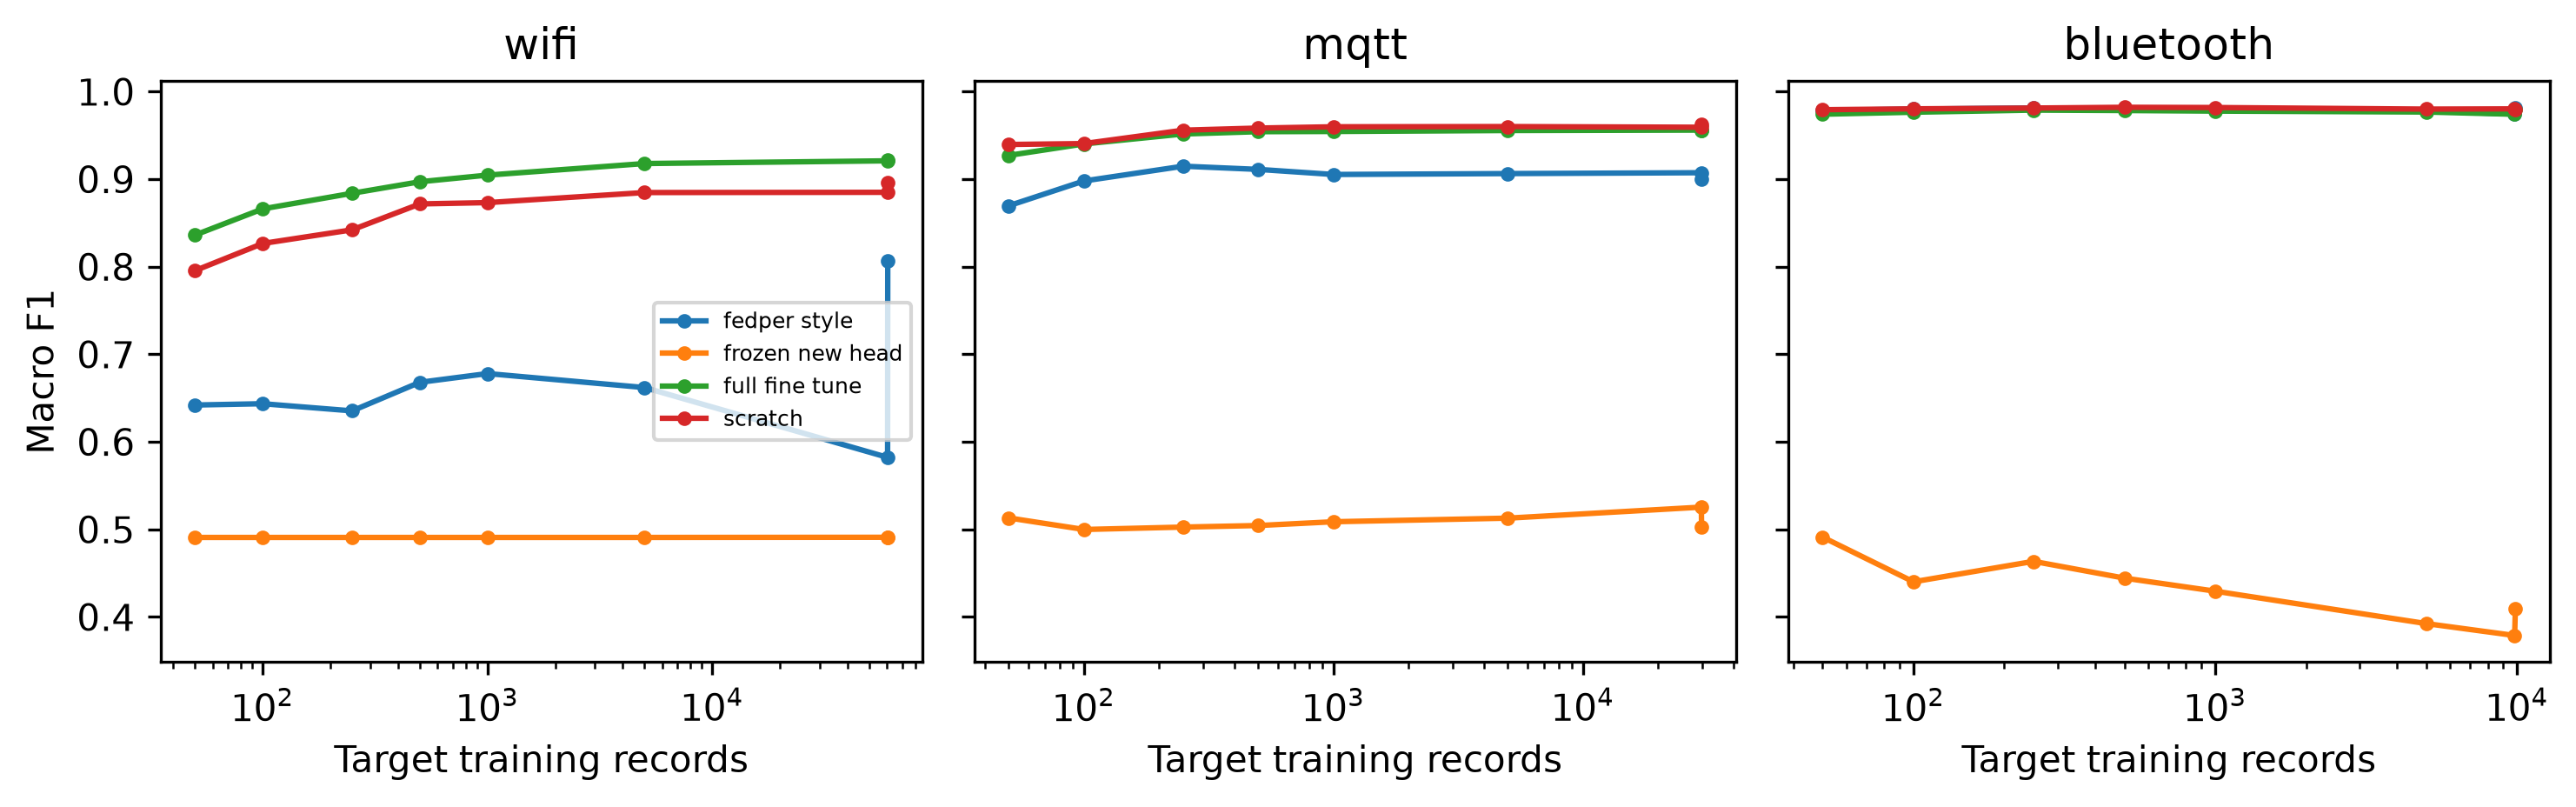
\includegraphics[width=0.93\textwidth]{revision_scarcity.png}
\caption{Target-excluded adaptation by budget and protocol. Full budgets can differ by seed.}\label{fig:revised_scarcity}
\end{figure*}
}

\history{Manuscript prepared for review.}\doi{pending assignment}

\title{FedXplain-IoMT: Diagnosing Cross-Protocol Explanation Divergence in Federated Intrusion Detection for Medical IoT}

\author{\uppercase{Swayam Swaroop Sahu}\authorrefmark{1}, 
\uppercase{Prakhar Sharma}\authorrefmark{1}, 
\uppercase{Geraldine Bessie Amali D}\authorrefmark{1}, 
and \uppercase{Kathiravan Srinivasan}\authorrefmark{1}, \IEEEmembership{Senior Member, IEEE}}

\address[1]{School of Computer Science and Engineering, Vellore Institute of Technology, Vellore 632014, India (e-mail: sahuswayamswaroop@gmail.com; prakhar.sharmaa2019@vitalum.ac.in; geraldine.amali@vit.ac.in; kathiravan.srinivasan@vit.ac.in)}

\markboth
{Sahu \headeretal: FedXplain-IoMT: Diagnosing Cross-Protocol Explanation Divergence}
{Sahu \headeretal: FedXplain-IoMT: Diagnosing Cross-Protocol Explanation Divergence}

\corresp{Corresponding author: Geraldine Bessie Amali D, Associate Professor Sr., School of Computer Science and Engineering, Vellore Institute of Technology, Vellore 632014, India (e-mail: geraldine.amali@vit.ac.in).}

\begin{abstract}
Client-averaged scores can conceal frequent false alarms on a particular communication protocol. We study this discrepancy in federated intrusion detection for the Internet of Medical Things using Wi-Fi, Message Queuing Telemetry Transport, and Bluetooth traffic. We keep identical feature vectors together when assigning training, validation, and test partitions and compare methods across \RevisionSeeds{} matched seeds. Federated averaging attained a client-mean macro F1 of \RevisionAvgF{} and Bluetooth benign recall of \RevisionAvgB{}. A private classification head raised Bluetooth benign recall to \RevisionPerB{}, and fixed protocol grouping raised it to \RevisionFixedB{}. The adaptive procedure selected separate groups for all clients. An equal-weight aggregation control also improved specificity. On frozen federated averaging models, a validation-fitted slope and intercept improved probability scores and specificity at a cost in attack recall. Positive temperature scaling improved probability scores while preserving the decisions. The mean absolute Shapley additive explanation rankings of two models remained highly correlated on the same Bluetooth records despite different operating points. These results describe one derived dataset and a fixed training schedule. Capture and device identities were unavailable, so evaluation on independent medical traffic remains open.
\end{abstract}
\begin{keywords}
Explainable artificial intelligence, federated learning, Internet of Medical Things, intrusion detection, model personalization, probability calibration.
\end{keywords}
\titlepgskip=-15pt
\maketitle
\section{Introduction}\label{sec:introduction}
\subsection{Clinical devices and network security}
\PARstart{A}{n} infusion pump delivers a programmed therapy while its network interface may carry configuration updates, status reports or alarms. An electrocardiography monitor samples continuously, a pulse oximeter sends oxygen saturation readings, and a smart bed may report occupancy or movement. The availability, freshness and origin of these messages matter for different reasons. A delayed oxygen alarm can leave a clinician looking at a stale value. An integrity failure can present a plausible but incorrect vital sign. A change to a pump configuration could affect dosage if authorization and device-level safeguards also failed. These are potential consequences. A flow-level attack label cannot establish that any occurred. Threat modeling of portable electrocardiography systems illustrates why the sensing device, gateway and monitoring application warrant separate analysis~\cite{ecg,trustreview,clinicalrisk}.

A network intrusion detection system (IDS) observes communication patterns. Traffic features can reveal unusual timing, excessive connection activity or changes in packet length without exposing the clinical payload. Encryption, shared gateways and intermittent connectivity limit what a detector can infer. Clinical triage therefore also requires device state and authentication logs. Resource-constrained anomaly detectors and specialized medical traffic models address different points in this monitoring pipeline~\cite{edgeids,specialized}.

\subsection{Federated learning and data locality}
An intrusion detector for the Internet of Medical Things (IoMT) can learn from extracted traffic features pooled across sites. The General Data Protection Regulation and the Health Insurance Portability and Accountability Act impose conditions on processing and disclosing identifiable health information~\cite{gdpr,hipaa2013security}. Federated learning (FL) allows sites to retain records while exchanging model parameters~\cite{nguyen2021federated,mcmahan2017communication}. An honest-but-curious aggregation service could inspect updates for information about participating clients~\cite{leakage}.

\subsection{Why global scores are insufficient}
Macro F1 gives the benign and attack classes equal weight within a client. Averaging again over clients produces one number for several distinct confusion matrices. A missed attack and a false alarm on a routine observation have different operational consequences. The harmonic means conceal how often either error occurs on a particular domain. We therefore report benign recall (specificity) and attack recall (sensitivity) for each client with the corresponding class supports.

\subsection{Protocol heterogeneity}
Wi-Fi conveys link-layer frames that can carry Internet Protocol (IP) traffic. The derived records include transport flags and service indicators. Message Queuing Telemetry Transport (MQTT) provides application-layer messaging over the Transmission Control Protocol (TCP). A client establishes a session with a broker and publishes or subscribes to topics. Repeated connection requests and heavy publication traffic can impose different costs on the broker. Bluetooth Low Energy (BLE) exchanges short link-layer payloads and can sleep between connection events. Their timing can reflect a wearable's duty cycle. The host-side Bluetooth captures expose controller packets and connection handles. The native Bluetooth records in this benchmark lack the IP headers available in the Wi-Fi records. Wi-Fi generally supports higher throughput, while Bluetooth wearables can prioritize energy per report. Specific bandwidth and battery use were not measured.

The benchmark includes Wi-Fi flooding, reconnaissance and spoofing, MQTT connection and publication floods and malformed messages, and Bluetooth denial of service (DoS)~\cite{dadkhah2024towards}. For example, broker overload can delay monitoring messages, while interrupted Bluetooth traffic can leave gaps in wearable observations. Table~\ref{tab:attacks} maps each retained label to its protocol and potential service impact. In the grouped experiments, Wi-Fi contributes the largest training partition and carries a high proportion of attack labels. Bluetooth has a benign majority. This creates differences in both class prevalence and client weight under sample-weighted aggregation.

FedXplain-IoMT evaluates established learning methods along three axes: class-specific detection, agreement of input attributions, and transfer to a client lacking particular local attack labels. We distinguish comparing traffic domains under one method from comparing models on the same domain. A separate output-level probe asks whether a fixed model can recover benign recall using only a local adjustment to its scores.

\subsection{Related Work}\label{sec:related_work}
Federated averaging (FedAvg) weights client updates by sample count~\cite{mcmahan2017communication}. Federated proximal optimization (FedProx) penalizes departure from broadcast weights~\cite{li2020federated}. Federated personalization layers (FedPer) retain selected parameters locally~\cite{arivazhagan2019federated}. Sattler and colleagues infer groups from update geometry~\cite{sattler2020clustered}. Our clustered baseline fixes groups before training.

The KDD Cup, UNSW-NB15, Bot-IoT and CICIoT2023 benchmarks cover different network environments~\cite{tavallaee2009detailed,moustafa2015unsw,koroniotis2019towards,neto2023ciciot2023}. Previous work combined federated intrusion detection and Shapley additive explanations (SHAP) on CICIoT2023 distributed across four clients~\cite{fedxai}. Here client membership follows traffic domain, and comparisons use binary-stratified record splits within each domain. We quantify how an explanation changes across domains or across models evaluated on one domain.

Graph-driven personalization learns relationships among clients, semi-decentralized training changes how participants exchange updates, and federated resampling changes the class distribution presented during training~\cite{graph,semidec,smote}. A distributed detector can also evaluate the cost of exchanging updates~\cite{hada}. Chandnani, Amali and colleagues study hyperparameter optimization for federated IoT intrusion detection~\cite{amali}. Here we hold architecture and training schedule fixed while comparing which parameters are shared.

Explainable detectors also use feature information at different stages. One distillation method uses Shapley additive explanations (SHAP) during learning~\cite{distill}, expert fusion organizes features into groups~\cite{experts}, and causal federated models introduce assumptions about relations among variables~\cite{causalfl}. Our post-hoc comparison leaves training unchanged. Its unit of analysis is a pair of model, client and sample configurations.

\begin{table*}[t]\caption{Examples of related evaluation scopes.}\label{tab:related}\centering
\begin{tabular}{p{.20\textwidth}p{.20\textwidth}p{.24\textwidth}p{.23\textwidth}}
\hline
Study & Data and heterogeneity & Learning or explanation & Scope\\\hline
Fatema et al.~\cite{fedxai} & CICIoT2023 client partitions & Federated classifier with post-training SHAP & Detection and feature importance\\
Graph personalization~\cite{graph} & Device and partition heterogeneity & Personalized graph-based detectors & Unsupervised detection\\
Feature-group fusion~\cite{experts} & CICIoMT2024 & Feature-group-aware expert fusion & Multi-class detection and interpretation\\
This study & Wi-Fi, MQTT and Bluetooth feature domains & Matched private-head, grouped and shared models & Within-client and cross-client explanation comparison and specificity diagnostics\\
\hline
\end{tabular}\end{table*}

\begin{table}[t]\caption{Selected intrusion-detection benchmark contexts.}\label{tab:datasets}\centering
\begin{tabular}{p{.30\columnwidth}p{.59\columnwidth}}\hline
Benchmark & Unit and collection setting\\\hline
KDD, UNSW-NB15~\cite{tavallaee2009detailed,moustafa2015unsw} & General network intrusion benchmarks\\
BoT-IoT, CICIoT2023~\cite{koroniotis2019towards,neto2023ciciot2023} & Botnet and broader Internet of Things traffic\\
Edge-IIoTset~\cite{edgeiio} & Edge and industrial Internet of Things traffic with distributed baselines\\
N-BaIoT~\cite{nbaiot} & Device measurements of botnet traffic\\
WUSTL EHMS~\cite{wustlehms} & Healthcare network flows and biometric observations\\
CICIoMT2024~\cite{dadkhah2024towards} & Multi-protocol medical-device testbed\\
\hline\end{tabular}\end{table}

\subsection{Research gap}
Results from separate benchmarks cannot by themselves identify the effect of a private head. Feature definitions, support for benign traffic, dependence between records and the unit of splitting vary across datasets. IoMT-TrafficData provides a complementary acquisition pipeline~\cite{iottraffic}. Sampling-aware detection and cross-domain transfer studies illustrate how the evaluation population changes the question~\cite{adaptive,transferstudy,drift}. We ask whether local specificity can change substantially when two models give similar aggregate attributions on the same records.

\subsection{Contributions}
\begin{itemize}
\item We compare federated baselines, personalization, grouping and aggregation controls with local-only and pooled training. We document split membership, label counts and exact feature overlap.
\item We apply private heads and fixed protocol groups to the same medical traffic partition. Our contribution is the evaluation of these established strategies against a local-only control under a common measurement protocol.
\item We separate cross-client and within-client explanations and test an output adjustment on frozen checkpoints. Transfer experiments include a source-matched benign control. Adaptation experiments compare target-excluded pretraining with training from scratch under matched update budgets.
\end{itemize}
\section{Dataset and Attack Taxonomy}
\subsection{Benchmark and partitions}\label{sec:data}
The Canadian Institute for Cybersecurity Internet of Medical Things 2024 (CICIoMT2024) benchmark comprises 25 physical and 15 simulated devices~\cite{dadkhah2024towards}. The derived Wi-Fi and MQTT tables were sampled from benchmark feature files. Bluetooth records were derived from Host Controller Interface (HCI) H4 captures. The historical extraction notes describe one-second windows and connection handles, along with zero-filled inapplicable Internet Protocol fields and a repurposed Logical Link Control feature. The feature dictionary records these mappings and states which units and extractor formulas remain unverified. The original capture-to-row manifest was unavailable, so the historical acquisition, filter and sampling steps could not be reconstructed exactly.

This revision assigns identical 45-feature vectors to the same group across all clients before partitioning. A grouped holdout selects test groups, and a separate grouped split selects validation groups from the remainder. Approximate target fractions are three fifths, one fifth, and one fifth for train, validation, and test. Group sampling can change the row proportions. The protocol shortcut experiment predicts client membership from documented inapplicable fields, encoded as zero or nonzero. This measures how strongly the schema encodes protocol membership.
\subsection{Attack labels and clinical interpretation}
The Canadian Institute for Cybersecurity grouped testbed traffic into denial of service, distributed denial of service (DDoS), reconnaissance, spoofing and MQTT scenarios. For Wi-Fi, the flood labels distinguish TCP, User Datagram Protocol (UDP), Internet Control Message Protocol (ICMP) and traffic with the TCP synchronization flag (SYN). The reconnaissance labels distinguish operating-system identification, host discovery, port enumeration and vulnerability scanning. Address Resolution Protocol (ARP) spoofing concerns the binding between an address and a local link endpoint. The MQTT scenarios distinguish session establishment, publication traffic and malformed messages. The Bluetooth DoS label identifies the source scenario without specifying an IP-layer mechanism. Table~\ref{tab:attacks} lists the retained source labels and their possible service consequences. Training maps those attack labels to a single positive class and evaluates benign traffic separately.

\RevisionTaxonomy

\subsection{Partitioning and prevalence}
Protocol prevalence and label support describe different forms of heterogeneity. The Wi-Fi partition has the largest sample count and the highest proportion of attacks. The Bluetooth partition contains a benign majority. The resulting distribution changes both the sample-weighted update mixture and the operational meaning of a global score. Table~\ref{tab:newsupport} gives train, validation, and test supports under one realized grouped partition.
\begin{figure}[t]\centering
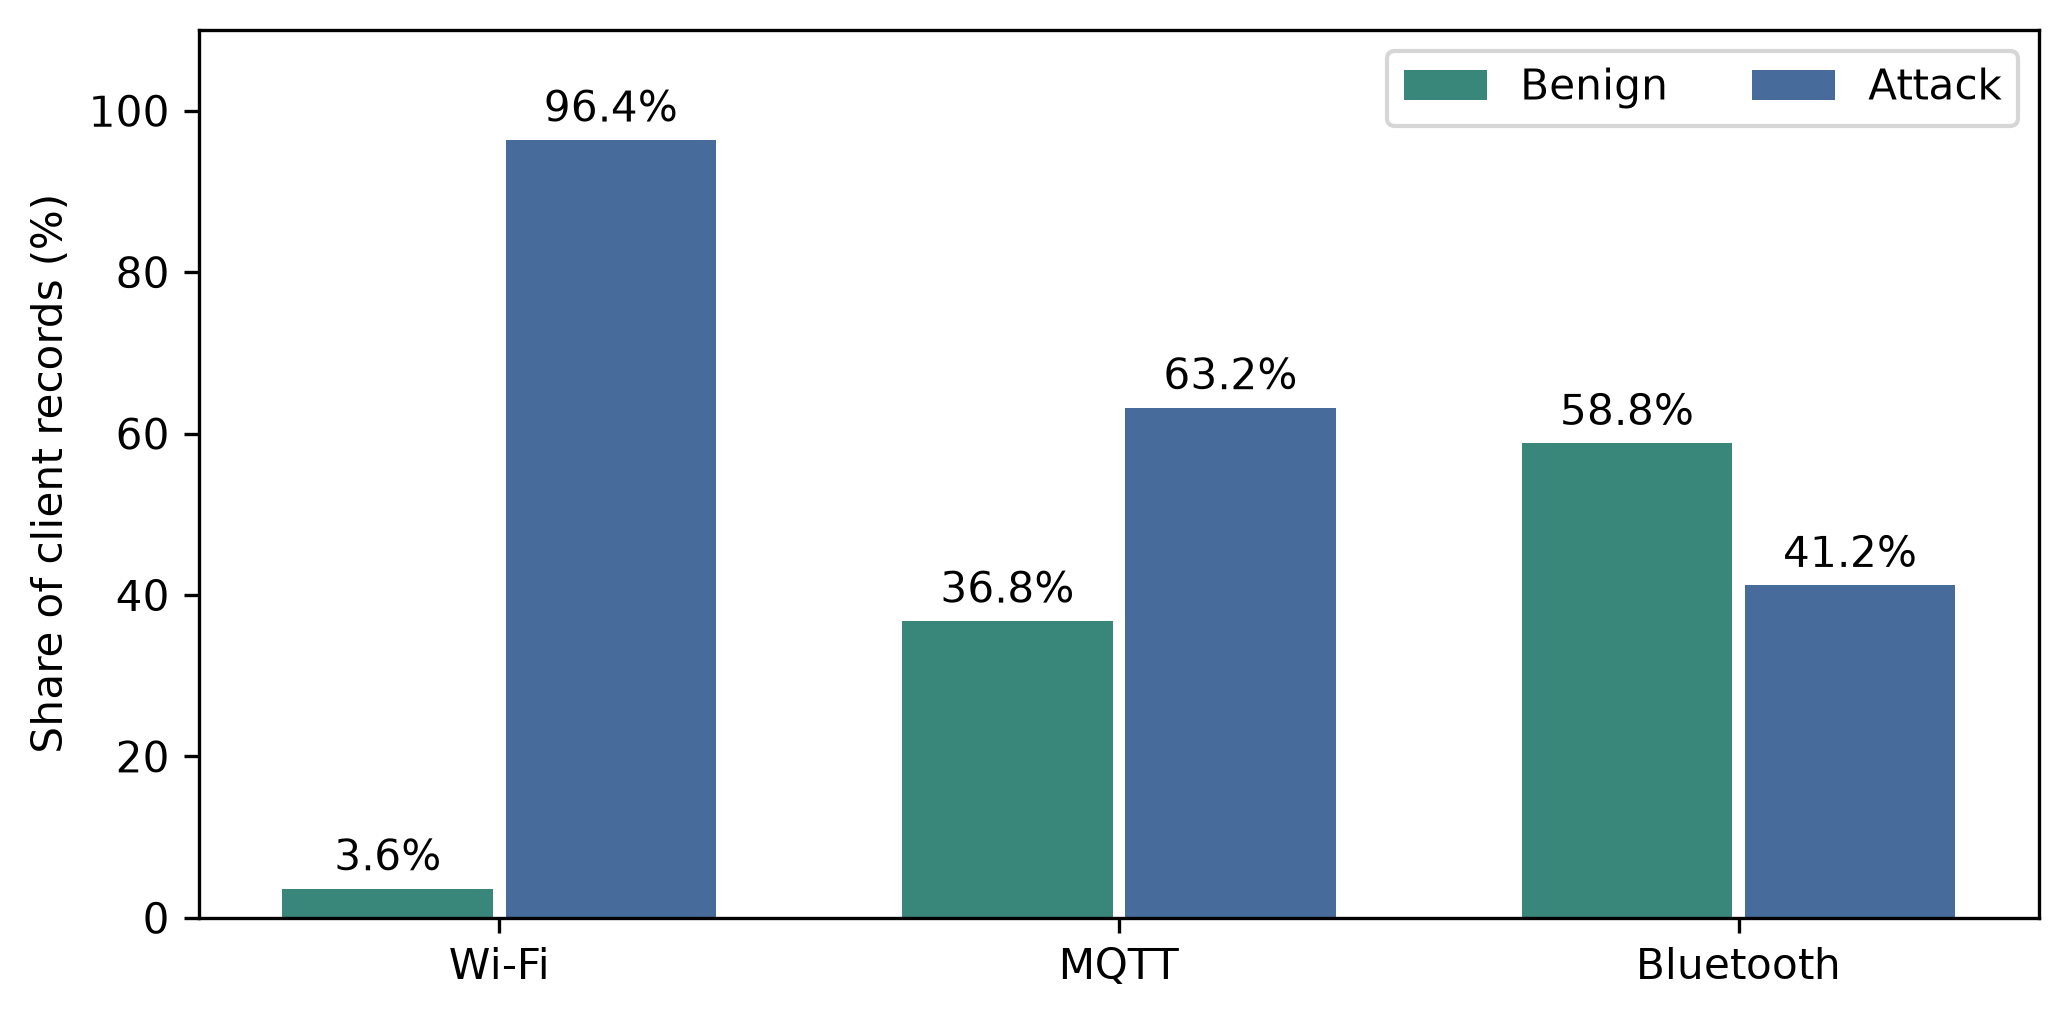
\includegraphics[width=\columnwidth]{fig_attack_distribution.png}
\caption{Benign and attack prevalence in the derived protocol tables.}\label{fig:attack_distribution}
\end{figure}

\section{System Architecture and Methodology}\label{sec:methods}
\subsection{Preprocessing, evaluation unit and threat model}
Nonfinite feature values map to zero before splitting. Train-only per-client standardization uses the mean $\boldsymbol{\mu}_k$ and scale $\boldsymbol{\sigma}_k$ of client $k$. Each evaluated record uses its target client's scaler. Thus a weight shared across clients acts on standardized values that can have different physical meanings. In the offline pooled comparator, the training input concatenates the client-standardized matrices and testing applies the scaler appropriate to each client. The grouping unit is an identical feature vector, rather than a verified capture or device. We screen near matches by rounding to four significant digits and counting signatures that occur across partitions.

The aggregation service follows the declared protocol and can observe the communicated parameters. The simulation does not model secure aggregation, differential privacy, poisoning defenses, or closed-loop clinical responses. This scope is compatible with an honest-but-curious server assumption.

\subsection{Multilayer perceptron and optimization}\label{sec:training}
The binary multilayer perceptron (MLP) in Fig.~\ref{fig:mlp} maps traffic features $\mathbf x\in\mathbb R^{45}$ to a single logit. Each client has a training set $\mathcal D_k=\{(\mathbf x_{ki},y_{ki})\}_{i=1}^{n_k}$ and $n=\sum_k n_k$. Labels $y\in\{0,1\}$ use one for attack. With rectified linear units (ReLU) acting elementwise,
\begin{align}
\mathbf h_1 &= \operatorname{ReLU}(W_1\mathbf x+\mathbf b_1),\\
\tilde{\mathbf h}_1 &= \operatorname{Dropout}(\mathbf h_1,\RevisionDropout),\\
\mathbf h_2 &= \operatorname{ReLU}(W_2\tilde{\mathbf h}_1+\mathbf b_2),\\
z &= W_3\mathbf h_2+b_3,\quad p=(1+\exp(-z))^{-1}.
\end{align}
Dropout acts as the identity during evaluation. The baseline decision is $\mathbb{1}\{z\geq0\}$. PyTorch computes minibatch-mean binary cross-entropy (BCE) from logits for numerical stability~\cite{paszke2019pytorch}. The equivalent local empirical objective is
\begin{equation}
f_k(w)=-\frac{1}{n_k}\sum_i [y_{ki}\log p_{ki}+(1-y_{ki})\log(1-p_{ki})].
\end{equation}
FedAvg broadcasts a common model in round $t$ before each client calculates its local fit $w_{k,t}$. It aggregates
\begin{equation}
w_{t+1}=\sum_k(n_k/n)w_{k,t}.
\end{equation}
FedProx adds a squared distance penalty on all trainable parameters to each local objective,
\begin{equation}
f_k(w)+\frac{\mu}{2}\|w-w_t\|_2^2.
\end{equation}
The same initialization and client-step seeds are used within each split. The zero-penalty control reproduces the FedAvg predictions. The class-balanced control instead weights each class inversely to its training frequency. The equal-weight control replaces the sample fractions by uniform client weights.

\begin{figure}[t]\centering
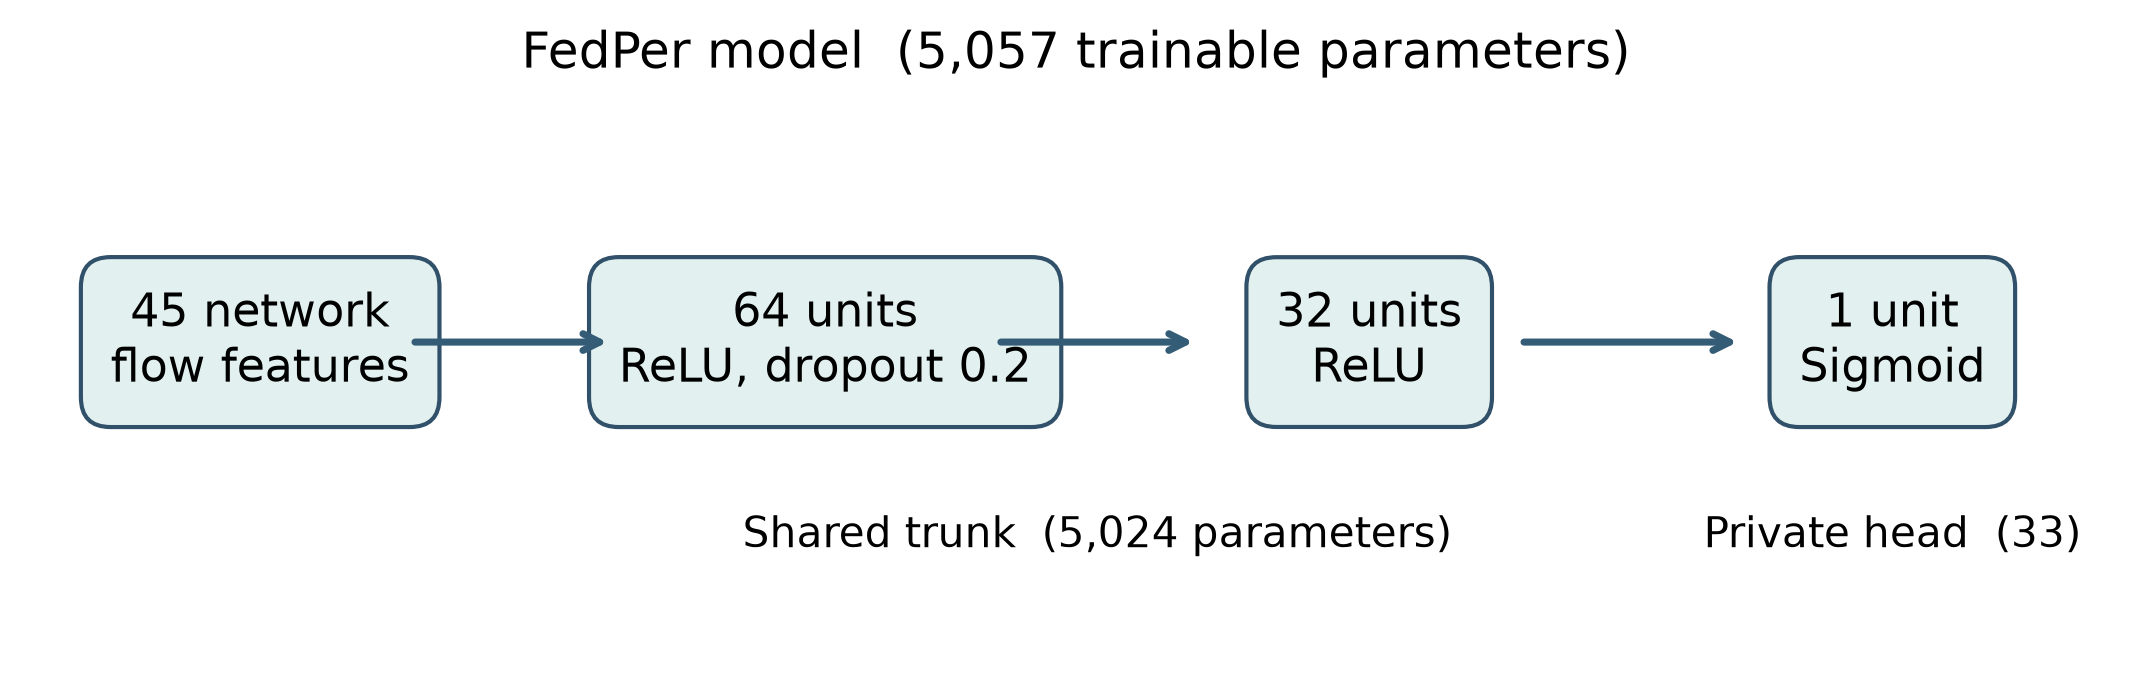
\includegraphics[width=\columnwidth]{fig_iomt_mlp_architecture.png}
\caption{MLP dimensions and the default FedPer parameter boundary.}\label{fig:mlp}
\end{figure}

\subsection{Private heads, fixed groups, and adaptive groups}
FedPer trains all local parameters but sends the trunk to the aggregator. Clients retain the head, including its bias, from one round to the next. At initialization every head comes from the same model within a seed. In the protocol-partitioned clustered baseline, Wi-Fi forms one group and MQTT and Bluetooth form the other. Each group averages the full model using its group-relative sample counts.

The adaptive comparator starts with all clients together. Following the norm-gated principle of clustered federated learning~\cite{sattler2020clustered}, we summarize the mean and maximum norms of the model updates within each group, relative to its initial update scale. After a configured warm-up, a low group-mean norm with a large individual norm triggers a split. Complete linkage uses distances equal to one minus the cosine of the update vectors. We use this finite-budget operational adaptation of the published procedure. Groups are then trained and evaluated independently. Table~\ref{tab:newgroups} and Fig.~\ref{fig:revised_topology} report the selected membership.

\RevisionTopology

\subsection{Training schedule and sensitivity design}
The main schedule uses \RevisionRounds{} rounds, \RevisionEpochs{} local epoch per round, minibatches of at most \RevisionBatch{}, and Adam learning rate \RevisionLr. All federated clients participate every round. Adam state resets for a fresh local federated fit. It persists across local-only blocks and pooled epochs. Matching the number of optimizer steps to the federated total defines the compute-matched central comparator. Matching steps does not equate communication, memory or data access. Pooled training is an empirical comparator. The legacy runner used the Flower interfaces~\cite{beutel2020flower}. The revised runner records each local update and its validation scores directly for all methods.

For each run, validation partitions select the checkpoint that minimizes the unweighted mean client BCE over logged snapshots. The selected checkpoint then produces the predictions for the held-out test partitions. The main series uses \RevisionSeeds{} matched seeds and all eligible records. We recompute detection metrics from the saved predictions, and the paper's tables, figures and numerical macros are generated from the run outputs. A separate two-seed grid changes local epochs, rounds, minibatch size, learning rate, dropout, hidden width and private head depth. Its round-by-epoch comparisons examine how those two scheduling choices interact within the tested grid. Main-run model selection uses only its own validation scores. Sensitivity, adaptation and reconnaissance-family withholding use seeds 42 and 7.

\subsection{Calibration diagnostics}
On Bluetooth each seed's validation groups are divided into separate fitting and selection sets. The fitting set supports a positive temperature, a logistic slope and intercept, a frozen-trunk head update, and a full-model update. The selection set chooses the head or full-model snapshots and the operating thresholds. The positive temperature applies $p_{\rm cal}=\sigma(z/T)$ with $T>0$ and preserves the sign of $z$~\cite{guocalibration}. An intercept can shift that sign. We compare the test operating points, Brier score and expected calibration error (ECE) from equal-width probability bins, and discrimination measured by the areas under receiver operating characteristic and precision--recall curves. A validation-selected low-false-positive operating point is evaluated on test at the same threshold. Linear centered kernel alignment (CKA) compares centered trunk activations across models on matching Bluetooth records~\cite{kornblithcka}.

\subsection{Attribution and detection metrics}\label{sec:metrics}
DeepExplainer estimates Shapley additive explanations (SHAP) for sigmoid probabilities in evaluation mode~\cite{lundberg2017unified}. On each client and seed, the background consists of up to \RevisionBg{} benign training records. We explain up to \RevisionSample{} records per class separately. FedAvg and FedPer use the same records and background within each client. Across clients the model, scaling, background distribution and evaluation population can differ. For each feature $j$ and fixed method, client and class,
\begin{equation}
\bar{\phi}_j=N_{\rm expl}^{-1}\sum_i |\phi_{ij}|.
\end{equation}
Top-five Jaccard similarity compares selected index sets with ties resolved by column order. With $\mathbf r_a,\mathbf r_b$ the centered average-rank vectors of two profiles,
\begin{align}
J(A,B)&=\frac{|T_5(A)\cap T_5(B)|}{|T_5(A)\cup T_5(B)|},\\
\rho(A,B)&=\frac{\mathbf r_a^\mathsf{T}\mathbf r_b}{\|\mathbf r_a\|\|\mathbf r_b\|},\\
C(A,B)&=\frac{A^\mathsf{T}B}{\|A\|\|B\|}.
\end{align}
The cosine lies in $[0,1]$ for nonnegative nonzero vectors. Zero and constant vectors make the relevant comparisons undefined. Within-client explanation intervals resample matched record indices, and across-client comparisons resample independently on each client. The sample bootstrap uses \RevisionBootstrap{} draws. An absolute inter-seed spread $|M_a-M_b|$ is descriptive. It is not an uncertainty threshold.

With attack as the positive class, TP, TN, FP and FN denote true positives, true negatives, false positives and false negatives. Benign recall is $\mathrm{TN}/(\mathrm{TN}+\mathrm{FP})$ and attack recall is $\mathrm{TP}/(\mathrm{TP}+\mathrm{FN})$. Client-mean macro F1 is the unweighted mean of the client binary macro F1 scores. Pooled macro F1 uses the combined confusion counts. Source-label recall tests whether the binary attack decision fires on each attack label. Attack-versus-benign precision limits the denominator to that attack label and benign test records. The model does not identify families.

\section{Results}\label{sec:results}
\subsection{Detection across traffic domains}
Tables~\ref{tab:newmain}, \ref{tab:newseed42} and \ref{tab:newseed7} report the aggregate and two reference splits. Across the \RevisionSeeds{} seeds, FedAvg attained client-mean macro F1 of \RevisionAvgF{} while recognizing only \RevisionAvgB{} of benign Bluetooth observations. FedPer reached \RevisionPerB{} and the protocol-partitioned clustered comparator reached \RevisionFixedB{}. Local-only training reached \RevisionLocalB{} and had strong detection on familiar client traffic. Centralized test F1 uses both the pooled and client-averaged definitions.

The adaptive procedure produced singleton groups at every validation-selected checkpoint. Thus its high Bluetooth specificity (\RevisionAdaptiveB{}) reflects separate client models at evaluation, with prior shared training. It offers evidence about the partition selected by this experiment. It supplies no evidence of a mutually beneficial learned protocol grouping under these settings.

When $R_{\rm local}>R_{\rm Avg}$, let $G=(R_{\rm Per}-R_{\rm Avg})/(R_{\rm local}-R_{\rm Avg})$ be the fraction of the benign-recall gap recovered on a fixed split. The individual scores in Tables~\ref{tab:newseed42} and \ref{tab:newseed7} provide these denominators. For seed 42, the paired percentile interval for the FedPer minus FedAvg specificity difference was $[\RevisionPerLo,\RevisionPerHi]$ under an exact-feature-group bootstrap. The unit is a feature-equivalence group, so the interval conditions on the observed partition and is not a device-level interval. Splits for different seeds can include many of the same observations. Seed-to-seed dispersion in Table~\ref{tab:newmain} is descriptive.

\RevisionDetection

\subsection{Regularization, update weights and budget}
Figure~\ref{fig:revised_sweep_budget} displays all tested proximal penalties for each seed. The penalties are discrete tested settings. The zero-penalty run reproduces FedAvg. Equal client weighting raised Bluetooth benign recall to \RevisionEqualB{}, while class balancing reached \RevisionBalancedB{}. These interventions alter different parts of optimization. The equal-weight result provides direct evidence that the aggregation rule matters for this training schedule. It does not isolate a unique mechanism from data prevalence, different numbers of client steps, or changing local models. The saved client update cosines are descriptive measures of model-update alignment, not gradients or causal effects.

Round-level validation loss and accuracy, step counts and elapsed training times accompany every run. The compute-matched central comparator uses the same optimizer step total as FedAvg. A descriptive plateau screen requires at least three evaluations in a final tail whose validation BCE range is at most $0.001$. We use the lowest validation BCE seen during the fixed schedule for selection and make no claim of reaching a stationary solution.

\RevisionBudget

\subsection{Output interventions and representation similarity}
Table~\ref{tab:newprobe} summarizes the Bluetooth probe. Starting from the same FedAvg scores, a validation-selected threshold raised mean specificity to \RevisionThresholdB{} with attack recall \RevisionThresholdA{}. Fitting a slope and intercept yielded specificity \RevisionPlattB{} and attack recall \RevisionPlattA{}, with a Brier improvement from \RevisionProbeAvgBrier{} to \RevisionPlattBrier{}. Temperature scaling changed the Brier score to \RevisionTemperatureBrier{} and preserved every binary decision. Thus changing probability calibration and changing an operating threshold are distinct actions. Full fine-tuning attained specificity \RevisionTuneB{} and attack recall \RevisionTuneA{}. The frozen-trunk head update improved specificity to \RevisionHeadB{} with attack recall \RevisionHeadA{}. The measured sensitivity--specificity trade-offs depend on which parameters are available for adjustment. Figure~\ref{fig:revised_diagnostic} illustrates these metrics and the FedAvg class-conditional score distributions.

FedAvg and FedPer had mean Bluetooth trunk CKA of \RevisionCka{} under matched test inputs. This indicates broad similarity of centered activation geometry. The same score does not imply that the decision-relevant directions, head parameters, or individual predictions coincide. In combination with the output-only and fine-tuning controls, the evidence supports multiple ways of improving the operating point on Bluetooth.

\RevisionDiagnostics

\subsection{Within-client and cross-client attributions}
In the Bluetooth within-client comparison, FedAvg and FedPer's mean absolute attribution ranks had mean Spearman correlations of \RevisionWithinAttack{} on attack records and \RevisionWithinBenign{} on benign records. The FedAvg attack comparison between Wi-Fi and Bluetooth was \RevisionAcrossAttack{}. The two comparisons use different evaluation populations. Table~\ref{tab:newshapwithin} compares models on matched client records, whereas Table~\ref{tab:newshapacross} compares clients within a method. Figure~\ref{fig:revised_shap_tradeoff} uses the all-pair average of the within-method attack correlations. Signed attributions, record IDs and sample-bootstrap intervals are saved for inspection. Similar rankings can coexist with different operating points and cannot establish representation invariance.

\RevisionShap

\subsection{Sensitivity and transfer}
Table~\ref{tab:newsensitivity} and Fig.~\ref{fig:revised_sensitivity} describe the observed contrasts on the reduced two-seed sensitivity budget. In the FedPer head-depth comparison, mean Bluetooth specificity was \RevisionHeadDepthOne{} with one private affine layer and \RevisionHeadDepthTwo{} when the final hidden layer and classifier were retained. This contrast motivates reporting the exact personalization boundary. The sensitivity grid does not select the main-run architecture.

For foreign-source transfer we apply each target's scaler and deployed head to test records from a different client. The benign flag rate comes from benign records of the same foreign source, and the detection margin is attack recall minus that flag rate. Table~\ref{tab:newtransfer} summarizes Bluetooth-target transfer. A separate two-seed experiment excludes the reconnaissance family from the training and validation records of all clients and fits all models and scalers anew. Table~\ref{tab:newholdout} reports recall on the held-out family. The test domain still comes from the same derived benchmark and can contain features shared with other attacks.

\RevisionSensitivity
\RevisionTransfer
\subsection{Target-excluded adaptation}
The budget is a count of target training records. On each budget the same stratified samples and update count are used for scratch training, a frozen trunk with a new head, two private layers with a frozen first layer, and full fine-tuning. Pretraining excludes the target client entirely. Each target scaler is fitted on the sampled budget. Figure~\ref{fig:revised_scarcity} shows that the best adaptation arm varies with the target and budget. The fixed step budget can restrict which sampled records are visited at the largest budgets.



\RevisionScarcity
\clearpage
\section{Discussion}\label{sec:discussion}
A high benign flag rate would impose review burden if a deployed monitor used the same scores and thresholds. For example, repeated alarms on routine wearable observations could delay review of other signals. The benchmark contains no observed patient outcomes. Client-specific false-positive rates and a separately selected operating point should be inspected before any containment action is considered.

The evidence comes from one subset and a simulated three-client federation, with lack of capture provenance and potential near duplicates. Across all revised partitions the exact-match count across splits was zero. The rounded signature screen still found possible near matches. A small classifier using only documented inapplicable fields predicted protocol identity with mean accuracy \RevisionShortcut\%. This illustrates a schema shortcut and does not quantify how much the intrusion detector itself relies on those fields. Bootstrap intervals condition on observed feature groups and omit independent capture variation. Transfer and adaptation remain offline evaluations.

SCAFFOLD uses first-order control variates to address client drift~\cite{karimireddy2020scaffold}, and FedNova normalizes local updates~\cite{wang2020tackling}. Those alternatives motivate further controls for effects of heterogeneous local work. Heterogeneity-aware methods can differ in which aspects of a training domain or feature schema they change. Our contribution is the matched evaluation of operating points, explanations and controls on these protocol partitions.

\section{Conclusion}\label{sec:conclusion}
FedAvg assigned many benign Bluetooth observations to the attack class under the evaluation schedule. Local heads, fixed groupings and equal weighting improved specificity under the matched comparison. Adaptive grouping yielded separate client models. A local score adjustment improved probability quality and changed the operating point, and full fine-tuning improved both recalls relative to Platt scaling. These findings are bounded by the feature-derived splits and compute schedule. Evaluation on independently collected captures remains necessary before deployment conclusions can be drawn.

\section*{Data and code availability}
The review bundle includes the feature schema, split manifest, experiment configuration, model checkpoints, predictions, numerical generation scripts, and summary artifacts. The original benchmark is available from the Canadian Institute for Cybersecurity~\cite{dadkhah2024towards}. The corresponding author will confirm the release identifier and licence.

\section*{Acknowledgment and declarations}
The authors will confirm acknowledgments, funding, competing interests and any applicable declarations before submission.

\bibliographystyle{IEEEtran}
\bibliography{refs/references}

\begin{IEEEbiography}[]{Swayam Swaroop Sahu}
is affiliated with the School of Computer Science and Engineering, Vellore Institute of Technology, Vellore, India.
\end{IEEEbiography}

\begin{IEEEbiography}[]{Prakhar Sharma}
is affiliated with the School of Computer Science and Engineering, Vellore Institute of Technology, Vellore, India.
\end{IEEEbiography}

\begin{IEEEbiography}[]{Geraldine Bessie Amali D}
is an Associate Professor Sr. at the School of Computer Science and Engineering, Vellore Institute of Technology, Vellore, India.
\end{IEEEbiography}

\begin{IEEEbiography}[]{Kathiravan Srinivasan}
is affiliated with the School of Computer Science and Engineering, Vellore Institute of Technology, Vellore, India. He is a Senior Member of the IEEE.
\end{IEEEbiography}

\EOD
\end{document}

